\documentclass{yThesis2}


% (*) Preparing figures:
% - dla linii 'lw 2' czyli grubosc 2, a dla error bars mozna zostawic domyslnie czyli (lw 1)
% - set terminal postscript eps enhanced color
% - najbardziej rozroznialne style: lt 1, 2, 3, etc. (do ustawienia stylu wystarczy 'lt x lw y' to ustawi kolor, rodzaj linii i grubosc
% - It looks that the best idea is to keep scaling=1.0 in latex all the time and then change the size in gnuplot only (e.g., set size 0.8, 0.8 in gnuplot). In this way all graphs have the same font size. Having this, one can produce figures of different sizes and font in all of them will be the same.
% - wszystkie skrypty do rozprawy beda mialy "\_thesis.plt" w koncowce nazwy


% this packages are for short citations in Latex
%\usepackage{dialogue}
%\usepackage{authordate1-4}
\usepackage{times}
\usepackage{setspace}
\usepackage[latin1]{inputenc}
\usepackage[UKenglish]{babel}
\usepackage{amsmath}
\usepackage{amsthm}
\usepackage{amssymb}
\usepackage{tabularx}
\usepackage{booktabs}
\usepackage{multirow}
\usepackage{subfigure}
\usepackage{verbatim}
\usepackage{float}
\usepackage{listings}
% to get the bibliography in the toc
\usepackage[nottoc,notlot,notlof,chapter]{tocbibind}
\usepackage{rotating}
\usepackage{titlesec}
\usepackage{url}
\usepackage{fancyhdr}
\usepackage{rst}
\usepackage{textcomp}
%\usepackage[greek,british]{babel}

%\usepackage{algorithms}
% \citet{jon90} ) Jones et al. (1990)
% \citet[chap.~2]{jon90} ) Jones et al. (1990, chap. 2)
% \citep{jon90} ) (Jones et al., 1990)
% \citep[chap.~2]{jon90} ) (Jones et al., 1990, chap. 2)
% \citep[see][]{jon90} ) (see Jones et al., 1990)
% \citep[see][chap.~2]{jon90} ) (see Jones et al., 1990, chap. 2)
% \citet*{jon90} ) Jones, Baker, and Williams (1990)
% \citep*{jon90} ) (Jones, Baker, and Williams, 1990)
% \citet{jon90,jam91} ) Jones et al. (1990); James et al. (1991)
% \citep{jon90,jam91} ) (Jones et al., 1990; James et al. 1991)
% \citep{jon90,jon91} ) (Jones et al., 1990, 1991)
% \citep{jon90a,jon90b} ) (Jones et al., 1990a,b)
\usepackage{natbib}
%\usepackage{makeidx}
%%index is better than makeindex as you can have more than one running
%%index file per document... this way, the author index is managed
%%separately
\usepackage{index}
%\usepackage{hyperref}
\usepackage[breaklinks=true]{hyperref}
\usepackage{qtree}
% The algorithm packages have to be after hyperref.
\usepackage{algorithm, algorithmic}
\usepackage{xspace, float, graphicx, pstricks}
\usepackage{wrapfig}
\usepackage[intoc,refpage]{nomencl} %refeq
\usepackage{longtable}
\usepackage{lscape}
\usepackage{slashbox}
%\usepackage{xfrac}
\makenomenclature

\usepackage{color}
\definecolor{javared}{rgb}{0.6,0,0} % for strings
\definecolor{javagreen}{rgb}{0.25,0.5,0.35} % comments
\definecolor{javapurple}{rgb}{0.5,0,0.35} % keywords
\definecolor{javadocblue}{rgb}{0.25,0.35,0.75} % javadoc
 
\lstset{language=Java,
basicstyle=\ttfamily,
keywordstyle=\color{javapurple}\bfseries,
stringstyle=\color{javared},
commentstyle=\color{javagreen},
morecomment=[s][\color{javadocblue}]{/**}{*/},
%numbers=left,
numberstyle=\tiny\color{black},
stepnumber=2,
numbersep=10pt,
tabsize=4,
showspaces=false,
showstringspaces=false}


\hypersetup{
   pdftitle = {New Strategies for Automated Random Testing},
   pdfsubject = {Ph.D. Thesis, The University of York},
   pdfkeywords = {phd, thesis, york, university, automated, random testing, YETI, software testing},
   pdfauthor = {\textcopyright\ \today\ Mian\'{s}},
   %pdfcreator = {\LaTeX\ with Emacs},
}


\setlength{\bibsep}{0pt}
\bibpunct[:]{(}{)}{;}{a}{}{,} % to format the way references are formatted inside the text
\renewcommand{\arraystretch}{1.17} % line spacing in tables
\setlength\tabcolsep{8pt} % column formatting in tables
\setcounter{tocdepth}{3} % how far the embedding goes in your TOC


\makeindex
%so natbib generates the author index
\citeindextrue
%so the author index is in an external citation file
%generate with:
%sed -e 's/{{\([^}]*\)}/{\1/g' main.adx > /tmp/main.adx; makeindex -s main.ist -o main.and /tmp/main.adx
\newindex{idx}{idx}{ind}{Index}
\newindex{aut}{adx}{and}{Citation Index}
\renewcommand{\citeindextype}{aut}


%%mark the things to do...
%\usepackage{color}
%\definecolor{Orange}{rgb}{1,0.5,0}
%\newcommand{\todo}[1]{\textsf{\textbf{\textcolor{Orange}{TODO [[#1]]}}}}
% Command for inserting a todo item
\usepackage{todonotes}
\reversemarginpar
\newcommand{\globaltodo}[1]{\addcontentsline{tdo}{todo}{Global: \protect{#1}}}
%\renewcommand{\todo}[1]{\todo[left]{#1}}
%%TODO%%
% (1) Type this: \listoftodos to generate a list of global TODOs
% (2) Each global TODO can be added in this way: \globaltodo{write here that to do}


% One of this too can be chosen.
%\usepackage[Bjornstrup]{fncychap}
\usepackage[Sonny]{fncychap}


\linespread{1.5}


% \makeglossary


\newtheorem{defin}{Definition}
\newtheorem{lemma}{Lemma}
\newtheorem{theor}{Theorem}


\title{New Strategies for\\[0.4cm]Automated Random Testing}
%\subtitle{Resources from Multilingual\\ Corpora and their
%Exploitation}
\author{Mian Asbat Ahmad}
\authoremail{mian.ahmad@york.ac.uk}
\dept{Department of Computer Science}
\submitdate{\today}


\begin{document}


% York reg 2.7.3 section l requires numbering from title page so \frontmatter can not be used.
% \onehalfspacing % looks better than double spacing, but \onehalfspacing is equivalent to \linespread{1.3}
% \mainmatter % is is necessary when the book class is used.


% % %%%%%%%%%%%%%%%%%%%%%% START HERE %%%%%%%%%%%%%%%%%%%%%%%%%%%%%%%%%%

\pagenumbering{roman}

% (1) The title page.
\titlePage

% (2) \correctionsPage

% (3) Abstract
\yabstract{
}

% (4) Table of contents, list of tables, list of figures.
\contents

% (5) Preface, if any, would go here.
%\preface{\input{preface}}

% (6) Acknowledgement
\acknowledgement{Several people have contributed to the completion of my PhD dissertation. However, the most prominent personality deserving due recognition is my worthy supervisor, Dr. Manuel Oriol. Thank you Manuel for your endless help, valuable guidance, constant encouragement, precious advice, sincere and affectionate attitude.

I thank my assessor Prof. John Clark for his constructive feedback on my various reports and presentations. I am also thankful and highly indebted to Prof. Richard Paige for his generous help, cooperation and guidance during my research at the University of York.

Special thanks to my father Prof. Mushtaq A. Mian who provided a conducive environment, valuable guidance and crucial support at all levels of my educational career and my very beloved mother whose love, affection and prayers have been my most precious assets. Also I am thankful to my elder brothers Dr. Ashfaq, Dr. Aftab, Dr. Ishaq, Dr. Afaq and my sister Dr. Haleema who have been the source of inspiration for me to pursue higher studies. My immediate younger brother Dr. Ilyas and my younger sister Ayesha studying in the UK, deserve recognition for their help, well wishes and moral support. Last but not the least I am very thankful to my dear wife Dr. Munazza for her company, help and cooperation throughout my stay at York.

I was funded by Departmental Overseas Research Scholarship (DORS), a financial support awarded to overseas students on the basis of outstanding academic ability and research potential. I am truly grateful to the Department of Computer Science for financial support that allowed me to concentrate on my research.
}

% (7) Declaration and published work.
\declaration{
This is a test message.
%\paragraph{Publications}

%\begin{figure}[b]
%\begin{center}
%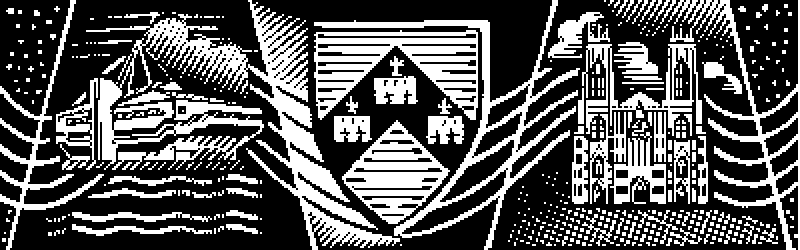
\includegraphics [width=7cm] {Woodcuts/univwoodcut}
%\end{center}
%\end{figure}
}

\newpage
\newpage
\newpage

\pagenumbering{arabic}

% (1.1) to whom: it goes to the second page immediately after the title page
\dedication{I feel it a great honour to dedicate my PhD thesis to my beloved parents for their significant contribution in achieving the goal of academic excellence reflected in my dissertation.
}

%%inroduction
\ychapter{Introduction and Motivation}{Introduction and
Motivation}{In this chapter we give a brief introduction and motivation for the research work presented in this thesis. We commence by introducing the problems in random testing. We then describe the alternative approaches to overcome these problems, followed by our research goals and contributions. At the end of the chapter, we give an outline of the thesis.

\section{The Problems}
In software testing, one is often confronted with the problem of selecting a test data set because exhaustive testing is not always applicable. Manual test data generation is a time-consuming and laborious exercise, therefore, automated test data generation is always preferred. Test data set is a subset of domain carefully selected to test the given software. Finding an adequate test data set is a crucial process in any testing technique as it aims to represent the whole infinite domain and evaluate the given system under test (SUT) for structural or functional properties \cite{mccabe1983} \cite{howden1986}. Test data generators are classified in to Pathwise, Goal-Oriented, Intellighent and Random \cite{wiki2013}. Random test data generation generate test data set randomly from the whole domain. Unlike other approaches Random approach is simple, easy to implement, fastest in computation and free from bias \cite{Ciupa2007}. \\ 
Despite the benefits random testing offers, its simplistic and non-systematic nature expose it to high criticism. \cite{Myers2004} mentioned it as "Probably the poorest methodology of all is random-input testing...". Where this statement is based on intuit n instead of experimental results but even if it is considered correct it is worth while to upgrade the strategy to generate more fault revealing test data. Random testing is also considered notorious for providing low code coverage \cite{Offutt1996}. For example, in random testing when the statement  ``if (x == 25) then ... "  is exposed to execution then there is only one chance, of the ``then..." part of the statement, to be executed out of $2^\text{32}$. If x is an integer variable of 32 bit value \cite{Godefroid2005}. Random testing is no exception when it comes to evaluate the results. Modern testing techniques deal with it by truncating the lengthy log files and display only the fault revealing test cases in the form of unit tests. However effort is required to show the test results in more compact and user friendly way. 


\section{Our Goals}
The overall goal of this thesis is to develop new techniques for automated testing based on random strategy that addresses the above mentioned problems. Particularly,

\begin{enumerate}
\item We aim to develop an automated testing technique which is able to generate more fault revealing test data out of the whole domain. In particular, it takes benefit of the presence of fault clusters found in the form of block and strip fault domains in the whole domain. Hence, we can automatically generate more fault revealing test data to evaluate the given SUT. Thus we are able to handle the problem of generating arbitrary data by random testing. 

\item We aim to develop a novel framework for finding the faults, their domains and their presentation on a graphical chart inside the specified lower and upper bound. It
considers the correlations of the fault and fault domain. It also gives a simplified and user friendly report to easily identify the faulty regions across the whole domain.

\item We aim to develop an automated strategy that utilises the literals of the SUT to particularly increase the total coverage and ultimately the overall results. On test initialisation it scan binary of the given SUT for literals. These literals are added to the prioritised list of interesting values to increase coverage and test performance. Thus we are able to handle the problem of coverage by random testing. 
\end{enumerate}

\section{Contributions}
To achieve the research goals described in Section xx, we make the following specific contributions:

\subsection{Dirt Spot Sweeping Random Strategy}
Development of a new, enhanced and improved form of automated random testing: the Dirt Spot Sweeping Random (DSSR) strategy. This strategy is based on the assumption that faults and unique failures reside in contiguous blocks and stripes. The DSSR strategy starts as a regular random+ testing strategy � a random testing technique with preference for boundary values. When a failure is found, it increases the chances of using neighbouring values of the failure in subsequent tests, thus slowly sweeping values around the failures found in hope of finding failures of different kind in its vicinity.
The DSSR strategy is implemented in the YETI random testing tool. It is evaluated against random (R) and random+ (R+) strategies by testing 60 classes (35,785 line of code) with one million (105) calls for each session, 30 times for each strategy. The results indicate that for 31 classes, all three strategies find the same unique failures. We analysed the 29 remaining classes using t-tests and found that for 7 classes DSSR is significantly better than both R+ and R, for 8 classes it performs similarly to R+ and is significantly better than R, and for 2 classes it performs similarly to ran- dom and is better than R+. In all other cases, DSSR, R+ and R do not perform significantly differently. Numerically, the DSSR strategy finds 43 more unique failures than R and 12 more unique failures than R+.

\subsection{Automated Discovery of Failure Domain}
There are several automated random strategies of software testing based on the presence of point, block and strip fault domains inside the whole input domain. As yet no particular, fully automated test strategy has been developed for the discovery and evaluation of the fault domains. We therefore have developed Automated Discovery of Failure Domain, a new random test strategy that finds the faults and the fault domains in a given system under test. It further provides visualisation of the identified pass and fail domain. In this paper we describe ADFD strategy, its implementation in YETI and illustrate its working with the help of an example. We report on experiments in which we tested error seeded one and two-dimensional numerical programs. Our experimental results show that for each SUT, ADFD strategy successfully performs identification of faults, fault domains and their representation on graphical chart.

\subsection{Random Plus Plus Strategy}
Acknowledgement of random testing being simple in implementation, quick in test case generation and free from any bias, motivated research community to do more for increase in performance, particularly, in code coverage and fault-finding ability. One such effort is Random+ --- Ordinary random testing technique with addition of interesting values (border values) of high preference. We took a step further in the same direction and developed Random++ strategy. Random++ strategy is an extended form of Random+ strategy with addition of program literals.  Literals from the given software under test are collected by instrumentation prior to testing and added to the list of interesting values.  Experimental result shows that Random++ not only increase the code coverage but also find some subtle errors that pure Random and Random+ were either unable or may take a long time to find.  



 
\section{Thesis Outline}

The rest of the thesis is organised as follows: In Chapter 2, we give a thorough review of the relevant literature. We commence by discussing a brief introduction of software testing and shed light on various techniques and types of software testing. Then, we extend our attention to automated random testing and the testing tools using random technique to test softwares. In Chapter 3, we present our first automated random strategy Dirt Spot Sweeping Random (DSSR) strategy based on sweeping faults from the clusters in the input domain. Chapter 4 describes our second automated random strategy which focus on dynamically finding the fault with their domains and its graphical representation. Chapter 5 presents the third strategy that focus on quick identification of faults and increase in coverage with the help of literals; Finally, in Chapter 7, we summarise the contributions of this thesis, discuss the weaknesses in the work, and suggest avenues for future work.






%Today, the primary focus of software companies is to achieve high quality. These companies spend an estimated thirty to ninety percent of the total software development cost on testing \ref{Beizer1990}, \ref{Standards2002}. In spite of spending 

%Software testing is the process of executing a software with specific test data followed by evaluation of the results to check whether it is working according to its specification or not \ref{Sommerville2006}.
% check here if we can replace specification with oracle or not.
%The test passes if the output complies to its specification and fails otherwise. The success of testing correlates with the number of failures found in the Software Under Test (SUT): a test is more successful if it finds more faults.

%It is interesting that program testing is used to show the presence of bugs, rather than absence of bugs [6]. Therefore the SUT that passes all the tests without returning a single failure does not guarantee that there is no fault. The testing process increases however the reliability and confidence of both the developers and the users in the tested product [7] [8] [9].

%Random testing is a black-box testing technique in which the SUT is executed against ran- domly selected test data. Test results obtained are compared either against the oracle defined, using SUT specifications in the form of assertions or exceptions defined by the programming language. The rapid increase in software development in today?s modern world prompts the need for automated testing to ensure high quality. The generation of random test data is com- paratively cheap and does not require too much intellectual and computation efforts [10] [11]. It is for this reason that various researchers have recommended this strategy for incorporation in automatic testing tools [12]. YETI [13] [14], AutoTest [15] [16], QuickCheck [17], Randoop [18], JArtage [19] are a few of the most common tools based on random strategy.
}


%%literature review
\ychapter{Literature Review}{Literature
Review\label{CHAP:FIELDREV}}{
\section{Software Testing}
\subsection{Categories of Software Testing}
\subsubsection{Black-box Testing}
\subsubsection{White-box Testing}
\subsection{Manual Testing}
\subsection{Automated Testing}
\subsubsection{Random Testing}
\subsubsection{Exhaustive Testing}

\section{Automated Random Testing}
\subsection{Test Data Generation}
\subsection{Test Execution}
\subsection{Test Oracle}
\subsection{Test Report}

\section{Variations is Random Testing}
\subsection{Adaptive Random Testing}
\subsection{Mirror Adaptive Random Testing}
\subsection{Directed Automated Random Testing}
\subsection{Quasi Random Testing}
\subsection{Monti Carlo Random Testing}
\subsection{Good Random Testing}
\subsection{Feedback-directed Random Testing}
\subsection{Adaptive Random Testing for Object-Oriented}
\subsection{Restricted Random Testing}

\section{Automated Random Testing Tools}
\subsection{JCrasher}
\subsection{JArtage}
\subsection{Eclat}
\subsection{JTest}
\subsection{QuickCheck}
\subsection{AgitarOne}
\subsection{Autotost}
\subsection{TestEra}
\subsection{Korat}
\subsection{RANDOOP}
\subsection{YETI}


\section{Conclusion}


}%{\input{FieldReview}}

%% The chapter on plan-based reward shaping.
%\ychapter{Design OR Title of the Paper}{Design OR Title of the
%Paper\label{CHAP:STRIPS}}{\input{STRIPS_Rshaping}}

%% The chapter on r-s from mixed resolution function approximation
\ychapter{Dirt Spot Sweeping Random Strategy}{Dirt Spot Sweeping Random Strategy\label{CHAP:DSSR}}{\section{Introduction}\label{sec:intro}
The success of a software testing technique is mainly based on the number of faults it discovers in the Software Under Test (SUT). An efficient testing process discovers the maximum number of faults in a minimum possible time. Exhaustive testing, where software is tested against all possible inputs, is mostly not feasible because of the large size of the input domain, limited resources and strict time constraints. Therefore, strategies in automated software testing tools are developed with the aim to select more fault-finding test input from input domain for a given SUT. Producing such targeted test input is difficult because each system has its own requirements and functionality.

Chan et al.~\cite{Chan1996} discovered that there are patterns of failure-causing inputs across the input domain. They divided the patterns into point, block and strip patterns on the basis of their occurrence across the input domain. Chen et al.~\cite{Chen2008} found that the performance of random testing can be increased by slightly altering the technique of test case selection. In adaptive random testing, they found that the performance of random testing increases by up to 50\% when test input is selected evenly across the whole input domain. This was mainly attributed to the better distribution of input which increased the chance of selecting inputs from failure patterns. Similarly Restricted Random Testing \cite{Chan2002}, Feedback directed Random Test Generation \cite{Pacheco2007a}, Mirror Adaptive Random Testing \cite{Chen2003} and Quasi Random Testing \cite{Chen2005} stress the need for test case selection covering the whole input domain to get better results.

In this paper we take the assumption that for a significant number of classes failure domains are contiguous or are very close by. From this assumption, we devised the Dirt Spot Sweeping\footnote{The name refers to the cleaning robots strategy which insists on places where dirt has been found in large amount.} Random (DSSR) strategy  which starts as a random+ strategy --- a random strategy focusing more on boundary values. When a new failure is found, it increases the chances of finding more faults using neighbouring values. As in previous studies~\cite{Oriol2012} we approximate faults with unique failures. Since this strategy is an extension of random testing strategy, it has the full potential to find all unique failures in the program, but additionally we expect it to be faster at finding unique failures, for classes in which failure domains are contiguous, as compared with random (R) and random+ (R+) strategies.

We implemented the DSSR strategy in the random testing tool YETI\footnote{\url{http://www.yetitest.org}}. To evaluate our approach, we tested 30 times each one of the 60 classes of 32 different projects from the Qualitas Corpus\footnote{\url{http://www.qualitascorpus.com}} with each of the three strategies R, R+ and DSSR. We observed that for 53\% of the classes all three strategies find the same unique failures, for remaining 47\% DSSR strategy perform up to 33\% better than random strategy and up to 17\% better than random+ strategy.
We also validated the approach by comparing the significance of these results using t-tests and found out that for 7 classes DSSR was significantly better than both R+ and R, for 8 classes DSSR performed similarly to R+ and significantly better than R, while in 2 cases DSSR performed similarly to R and significantly better than R+. In all other cases, DSSR, R+ and R do not seem to perform significantly differently.
Numerically, the DSSR strategy found 43 more unique failures than R and 12 more unique failures than R+ strategy. 

The rest of this paper is organised as follows: \\ Section~\ref{sec:dssr} describes the DSSR strategy. Section~\ref{sec:imp} presents implementation of the DSSR strategy. Section~\ref{sec:eval} explains the experimental setup. Section~\ref{sec:res} shows results of the experiments. Section~\ref{sec:discussion} discusses the results. Section~\ref{sec:rw} presents related work and Section~\ref{sec:conc}, concludes the study.




%%%%%%%%%%%%%%%%%    DIRT SPOT SWEEPING STRATEGY  %%%%%%%%%%%%%%%

\section{Dirt Spot Sweeping Random Strategy}\label{sec:dssr}
The new software testing technique named, Dirt Spot Sweeping Random (DSSR) strategy combines the random+ strategy with a dirt spot sweeping functionality. It is based on two intuitions. First, boundaries have interesting values and using these values in isolation can provide high impact on test results. Second, faults and unique failures reside in contiguous block and strip pattern. If this is true, DSS increase the performance of the test strategy. Before presenting the details of the DSSR strategy, it is pertinent to review briefly the Random and the Random+ strategy.

\subsection{Random Strategy (R)}
The random strategy is a black-box testing technique in which the SUT is executed using randomly selected test data. Test results obtained are compared to the defined oracle, using SUT specifications in the form of contracts or assertions. In the absence of contracts and assertions the exceptions defined by the programming language are used as test oracles. Because of its black-box testing nature, this strategy is particularly effective in testing softwares where the developers want to keep the source code secret~\cite{Chen2010}. The generation of random test data is comparatively cheap and does not require too much intellectual and computational efforts~\cite{Ciupa2009, Ciupa2008}. It is mainly for this reason that various researchers have recommended random strategy for automated testing tools \cite{Ciupa2008a}. YETI \cite{Oriol2010a, Oriol2010}, AutoTest \cite{Leitner2007, Ciupa2007}, QuickCheck \cite{Claessen2000}, Randoop \cite{Pacheco2007}, JArtege \cite{Oriat2004} are some of the most common automated testing tools based on random strategy.

\indent Efficiency of random testing was made suspicious with the intuitive statement of Myers \cite{Myers2004} who termed random testing as one of the poorest methods for software testing. However, experiments performed by various researchers, \cite{Ciupa2007, Duran1981, Duran1984, Hamlet1994, Ntafos2001} have proved experimentally that random testing is simple to implement, cost effective, efficient and free from human bias as compared to its rival techniques.

Programs tested at random typically fail a large number of times (there are a large number of calls), therefore, it is necessary to cluster failures that likely represent the same fault. The traditional way of doing it is to compare the full stack traces and error types and use this as an equivalence class~\cite{Ciupa2007,Oriol2012} called a unique failure. This way of grouping failures is also used for random+ and DSSR.

\subsection{Random Plus Strategy (R+)}
The random+ strategy~\cite{Leitner2007} is an extension of the random strategy. It uses some special pre-defined values which can be simple boundary values or values that have high tendency of finding faults in the SUT. Boundary values~\cite{Beizer1990} are the values on the start and end of a particular type. For instance, such values for \verb+int+ could be \verb+MAX_INT+, \verb+MAX_INT-1+, \verb+MAX_INT-2+; \verb+MIN_INT+, \verb-MIN_INT+1-, \verb-MIN_INT+2-. Similarly, the tester might also add some other special values that he considers effective in finding faults for the SUT. For example, if a program under test has a loop from -50 to 50 then the tester can add -55 to -45, -5 to 5 and 45 to 55 to the pre-defined list of special values. This static list of interesting values is manually updated before the start of the test and has slightly high priority than selection of random values because of more relevance and high chances of finding faults for the given SUT. These special values have high impact on the results, particularly for detecting problems in specifications~\cite{Ciupa2008}.


\subsection{Dirt Spot Sweeping (DSS)}
Chan et al.~\cite{Chan1996} found that there are patterns of failure-causing inputs across the input domain. Figure \ref{fig:patterns} shows these patterns for two dimensional input domain. They divided these patterns into three types called points, block and strip patterns. The black area (points, block and strip) inside the box show the input which causes the system to fail while white area inside the box represent the genuine input. Boundary of the box (black solid line) surrounds the complete input domain and represents the boundary values. They argue that a strategy has more chances of hitting these fault patterns if test cases far away from each other are selected. Other researchers~\cite{Chan2002, Chen2003, Chen2005}, also tried to generate test cases further away from one another targeting these patterns and achieved better performance. Such increase in performance indicate that faults more often occur contiguous across the input domain. In Dirt Spot Sweeping we propose that if a value reveals fault from the block or strip pattern then for the selection of the next test value, DSS may not look farthest away from the known value and rather pick the closest test value to find another fault from the same region.

\begin{figure}[ht]                                    
\centering
\includegraphics[width= 8cm,height=2.5cm]{DSSR/ART_Patterns.png}
\caption{Failure patterns across input domain~\cite{Chen2008}}
\label{fig:patterns}
\end{figure}

Dirt spot sweeping is the part of DSSR strategy that comes into action when a failure is found in the system. On finding a failure, it immediately adds the value causing the failure and its neighbouring values to the existing list of interesting values. For example, in a program when the \verb+int+ type value of 50 causes a failure in the system then spot sweeping will add values from 47 to 53 to the list of interesting values. If the failure lies in the block or strip pattern, then adding it's neighbouring values will explore other failures present in the block or strip. As against random plus where the list of interesting values remain static, in DSSR strategy the list of interesting values is dynamic and changes during the test execution of each program.

\begin{figure}[ht]
\centering
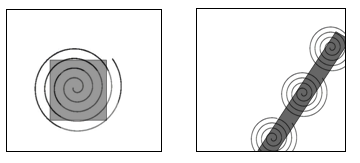
\includegraphics[width=8cm,height=2.2cm]{DSSR/block2.png}
\caption{DSSR covering block and strip pattern}
\label{fig:block2}
\end{figure}

Figure \ref{fig:block2} shows how DSS explores the failures residing in the block and strip patterns of a program. The coverage of block and strip pattern is shown in spiral form because first failure leads to second, second to third and so on till the end. In case the failure is positioned on the point pattern then the added values may not be effective because point pattern is only an arbitrary failure point in the whole input domain.

\subsection{Structure of the Dirt Spot Sweeping Random Strategy}

The DSSR strategy continuously tracks the number of failures during the execution of the test. This tracking is done in a very effective way with zero or minimum overhead to keep the overhead up to bare minimum~\cite{Leitner2009}. The test execution is started by R+ strategy and continues till a failure is found in the SUT after which the program copies the values leading to the failure as well as the surrounding values to the variable list of interesting values. 

\begin{figure}[ht]
\centering
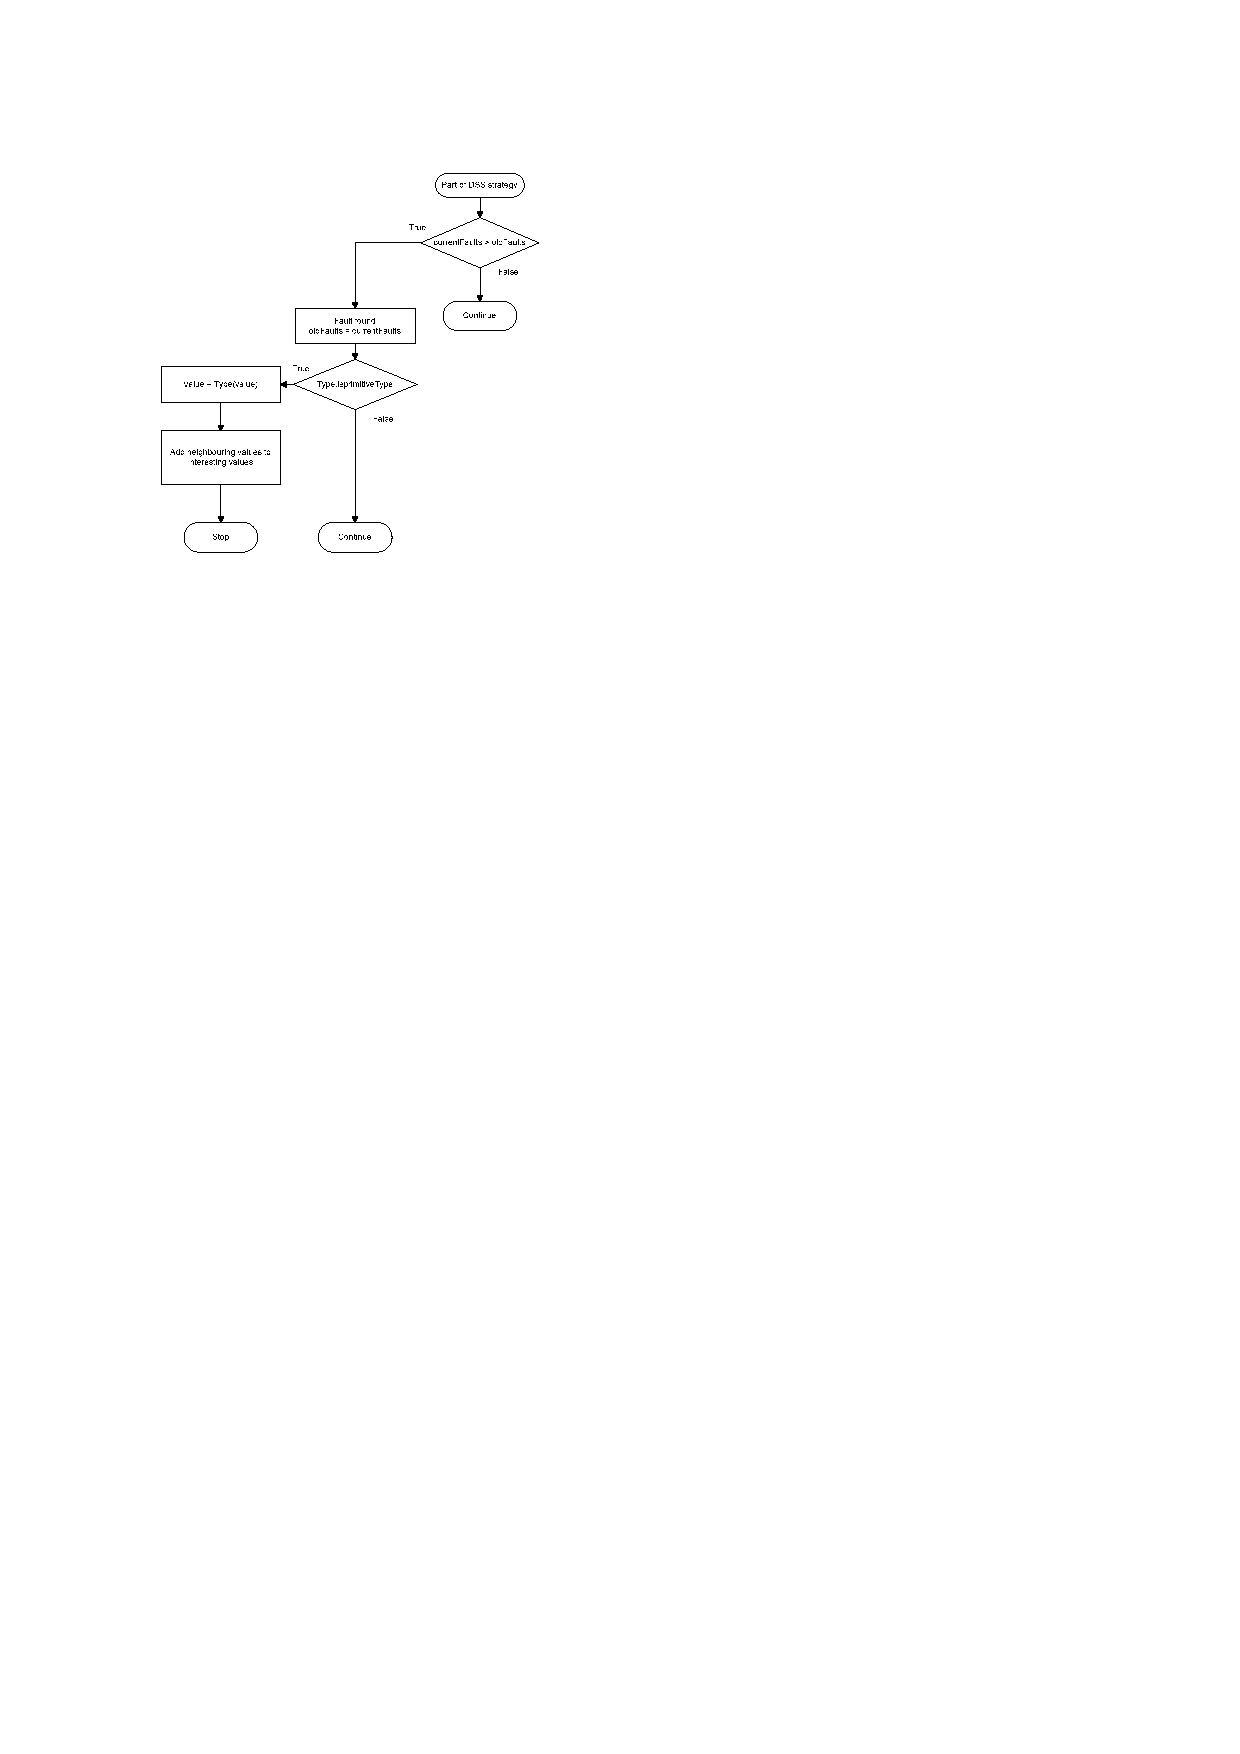
\includegraphics[width=\columnwidth]{DSSR/flowchart1.pdf}
\caption{Working mechanism of DSSR Strategy}
\label{fig:Working_DSSS}
\end{figure}

The flowchart presented in Figure~\ref{fig:Working_DSSS} depicts that, when the failure finding value is of primitive type, the DSSR strategy identifies its type and add values only of that particular type to the list of interesting values. The resultant list of interesting values provide relevant test data for the remaining test session and the generated test cases are more targeted towards finding new failures around the existing failures in the given SUT.

Boundary and other special values that have a high tendency of finding faults in the SUT are added to the list of interesting values by random+ strategy prior to the start of test session where as in DSSR strategy the fault-finding and its surrounding values are added at runtime when a failure is found. 

Table \ref{table:addvalues} presents the values are added to the list of interesting values when a failure is found. In the table the test value is represented by X where X can be int, double, float, long, byte, short, char and String. All values are converted to their respective types before adding them to the list of interesting values.

\begin{table}[ht]
%\scriptsize
\caption{Neighbouring values for primitive types and String} % title of Table
\centering % used for centering table
\begin{tabular}{| l | l |} % centered columns (4 columns)
\hline\hline %inserts double horizontal lines
Type & Values to be added\\ [0.5ex] % inserts table
%heading
\hline % inserts single horizontal line
\multirow{1}{*}{X is int, double, float, } & ~ X,  X+1, X+2, X-1, X-2 \\ % inserting body of the
\multirow{1}{*}{long, byte, short \& char} &  \\ 

\hline
\multirow{8}{*}{X is String} & ~ X\\ % inserting body of the table

& ~ X + ``  "\\ % inserting body of the table
& ~ ``  " + X \\ % inserting body of the table
& ~ X.toUpperCase() \\
& ~ X.toLowerCase() \\
& ~ X.trim() \\
& ~ X.substring(2) \\
& ~ X.substring(1, X.length()-1) \\[1ex]
\hline
\hline %inserts single line
\end{tabular}
\bigskip
\label{table:addvalues} % is used to refer this table in the text
\end{table}





%%%%%%%%%%%%%%%%%%%%%%%%%%%%% EXPLANATION OF DSSR STRATEGY %%%%%%%%%%%%%%%%%%%%%%%%%%


\subsection{Explanation of DSSR strategy on a concrete example}
The DSSR strategy is explained through a simple program seeded with three faults. The first fault is a division by zero exception denoted by 1 while the second and third faults are failing assertion denoted by 2 and 3 in the given program below followed by description of how the strategy perform execution.

\begin{lstlisting}
/** 
* Calculate square of given number 
* and verify results. 
* The code contain 3 faults.
* @author (Mian and Manuel)
*/
public class Math1 {
 public void calc (int num1) {
  // Square num1 and store result. 
  int result1 = num1 * num1;
  int result2 = result1 / num1; // 1
  assert Math.sqrt(result1) == num1; // 2
  assert result1 >= num1; // 3
 } 
}
\end{lstlisting}

In the above code, one primitive variable of type \verb+int+ is used, therefore, the input domain for DSSR strategy is from \verb+-2,147,483,648 to 2,147,483,647+. The strategy further select values (\verb+0, Integer.MIN_VALUE+ \& \verb+Integer.MAX_VALUE+) as interesting values which are prioritised for selection as inputs. 
As the test starts, three faults are quickly discovered by DSSR strategy in the following order.

\indent \textbf{Fault 1:} The strategy select value \verb+0+ for variable \verb+num1+  in the first test case because \verb+0+ is available in the list of interesting values and therefore its priority is higher than other values. This will cause Java to generate division by zero exception (1).

\indent \textbf{Fault 2:} After discovering the first fault, the strategy adds it and its surrounding values to the list of interesting values i.e. \verb+0, 1, 2, 3 and -1, -2, -3+ in this case. In the second test case the strategy may pick \verb+-3+ as a test value which may lead to the second fault where assertion (2) fails because the square root of \verb+9+ is \verb+3+ instead of the input value -3.

\indent \textbf{Fault 3:} After a few tests the strategy may select \\ \verb+Integer.MAX_VALUE+ for variable \verb+num1+  from the list of interesting values leading to discovery of the 3rd fault because int variable \verb+result1+ will not be able to store the square of \\ \verb+Integer.MAX_VALUE+. Instead of the actual square value Java assigns a negative value (Java language rule) to variable result1 that will lead to the violation of the next assertion (3).

The above process explains that including the border, fault-finding and surrounding values to the list of interesting values in DSSR strategy lead to the available faults quickly and in fewer tests as compared to random and random+ strategy. R and R+ takes more number of tests and time to discover the second and third faults because in these strategies the search for new unique failures starts again randomly in spite of the fact that the remaining faults are very close to the first one.


%%%%%%%%%%%%%%%%%    IMPLEMENTATION OF DSSR STRATEGY   %%%%%%%%%%%%


\section{Implementation of the DSSR \\ strategy}\label{sec:imp}

Implementation of the DSSR strategy is made in the YETI open-source automated random testing tool. YETI, coded in Java language, is capable of testing systems developed in procedural, functional and object-oriented languages. Its language-agnostic meta model enables it to test programs written in multiple languages including Java, C\#, JML and .Net. The core features of YETI include easy extensibility for future growth, high speed ( up to one million calls per minute on java code), real time logging, real time GUI support, capability to test programs with multiple strategies and auto generation of test report at the end of test session. For large-scale testing there is a cloud-enabled version of YETI, capable of executing parallel test sessions in Cloud~\cite{Oriol2010}. A number of hitherto faults have successfully been found by YETI in various production softwares~\cite{Oriol2011, Oriol2012}.

YETI can be divided into three decoupled main parts: the core infrastructure, language-specific bindings and strategies. The core infrastructure contains representation for routines, a group of types and a pool of specific type objects. The language specific bindings contain the code to make the call and process the results. The strategies define the procedure of selecting the modules (classes), the routines (methods) and generation of values for instances involved in the routines. By default, YETI uses the random strategy if no particular strategy is defined during test initialisation. It also enables the user to control the probability of using null values and the percentage of newly created objects for each test session. YETI provides an interactive Graphical User Interface (GUI) in which users can see the progress of the current test in real time. In addition to GUI, YETI also provides extensive logs of the test session for more in-depth analysis.

The DSSR strategy is an extension of YetiRandomPlusStrategy, an extended form of the YetiRandomStrategy. The class hierarchy is shown in Figure \ref{fig:hierarchyofDSSR}.

\begin{figure}[h]
\centering
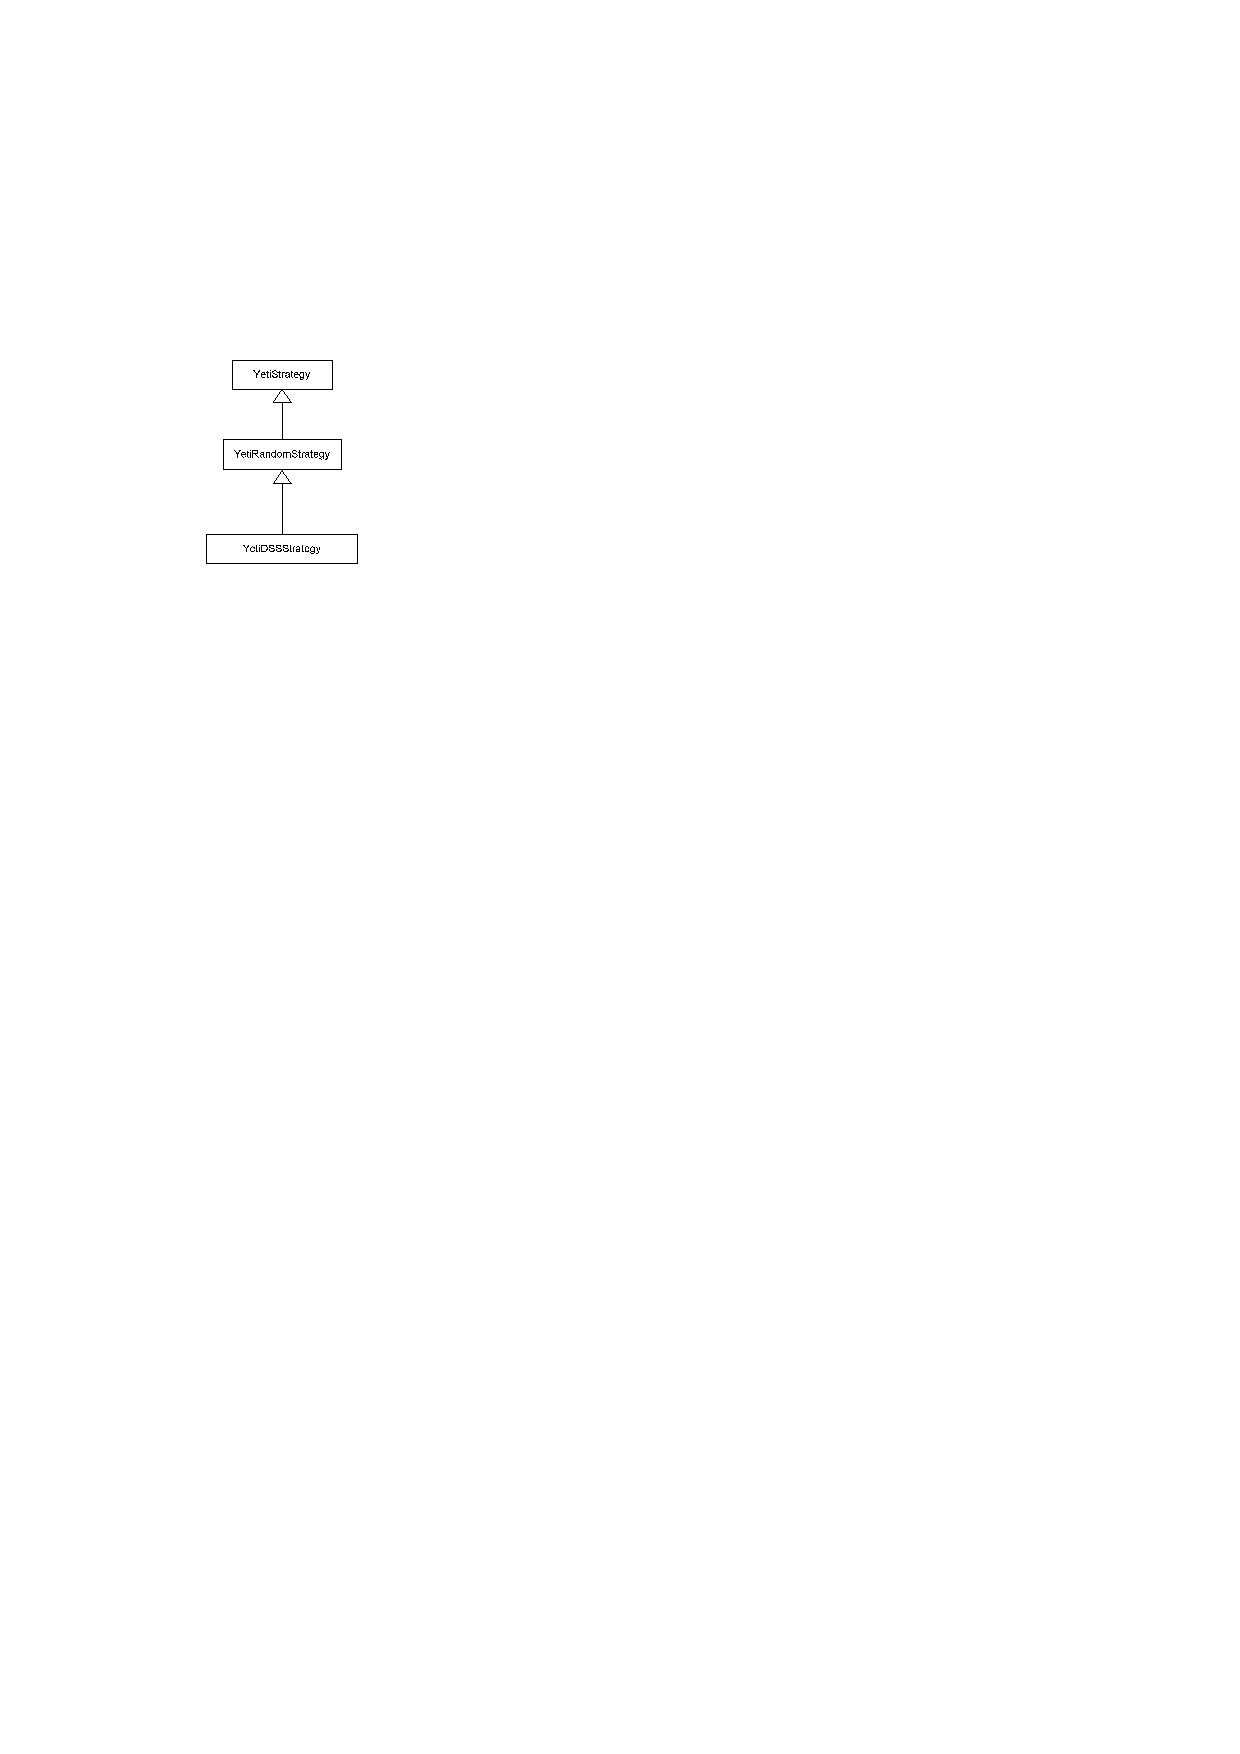
\includegraphics[width=4cm,height=5cm]{DSSR/hierarchy.pdf}
\caption{Class Hierarchy of DSSR in YETI}
\label{fig:hierarchyofDSSR}
\end{figure}





%%%%%%%%%%%%%%%%%    EVALUATION   %%%%%%%%%%%%%%%%%%%%


\section{Evaluation}\label{sec:eval}

The DSSR strategy is experimentally evaluated by comparing its performance with that of random and random+ strategy ~\cite{Leitner2007}. General factors such as system software and hardware, YETI specific factors like percentage of null values, percentage of newly created objects and interesting value injection probability have been kept constant in the experiments.

\subsection{Research questions}
For evaluating the DSSR strategy, the following research questions have been addressed in this study:
\begin{enumerate}
\item Is there an absolute best among R, R+ and DSSR strategies?
\item Are there classes for which any of the three strategies provide better results?
\item Can we pick the best default strategy between R, R+ and DSSR?
\end{enumerate}



\subsection{Experiments}

To evaluate the performance of DSSR we performed extensive testing of programs from the Qualitas Corpus~\cite{Tempero2010a}. The Qualitas Corpus is a curated collection of open source java projects built with the aim of helping empirical research on  software engineering. These projects have been collected in an organised form containing the source and binary forms. Version 20101126, which contains 106 open source java projects is used in the current evaluation. In our experiments we selected 60 random classes from 32 random projects. All the selected classes produced at least one fault and did not time out with maximum testing session of 10 minutes. Every class is tested thirty times by each strategy (R, R+, DSSR). Name, version and size of the projects to which the classes belong are given in table~\ref{table:projects} while test details of the classes is presented in table~\ref{table:Results}. Line of Code (LOC) tested per class and its total is shown in column 3 of table~\ref{table:Results}. 

Every class is evaluated through $10^5$ calls in each test session.\footnote{The total number of tests is thus $60\times 30\times 3 \times 10^5 = 540\times 10^6~tests$.} 
Because of the absence of the contracts and assertions in the code under test, Similar approach as used in previous studies ~\cite{Oriol2012} is followed using undeclared exceptions to compute unique failures.


\begin{table}[h]
\caption{Name and versions of 32 Projects randomly selected from the Qualitas Corpus for the experiments}
\centering
\begin{tabular}{|r|l|r|r|}
\hline
S. No& 	Project Name	& 	Version		&	Size (MB)\\
\hline
1	&	apache-ant	&	1.8.1			&	59\\
2	&	antlr			&	3.2			&	13\\
3	&	aoi			&	2.8.1			&	35\\
4	&	argouml		&	0.30.2		&	112\\
5	&	artofillusion	&	281			&	5.4\\
6	&	aspectj		&	1.6.9			&	109.6\\
7	&	axion		&	1.0-M2		&	13.3\\
8	&	azureus		&	1			&	99.3\\
9	&	castor		&	1.3.1			&	63.2\\
10	&	cayenne		&	3.0.1			&	4.1\\
11	&	cobertura		&	1.9.4.1		&	26.5\\
12	&	colt			&	1.2.0			&	40\\
13	&	emma		&	2.0.5312		&	7.4\\
14	&	freecs		&	1.3.20100406	&	11.4\\
15	&	hibernate		&	3.6.0			&	733\\
16	&	hsqldb		&	2.0.0			&	53.9\\
17	&	itext			&	5.0.3			&	16.2\\
18	&	jasml		&	0.10			&	7.5 \\
19	&	jmoney		&	0.4.4			&	5.3\\
20	&	jruby			&	1.5.2			&	140.7\\
21	&	jsXe			&	04\_beta		&	19.9\\
22	&	quartz		&	1.8.3			&	20.4\\
23	&	sandmark		&	3.4			&	18.8\\
24	&	squirrel-sql	&	3.1.2			&	61.5\\
25	&	tapestry		&	5.1.0.5		&	69.2\\
26	&	tomcat		&	7.0.2			&	24.1\\
27	&	trove			&	2.1.0			&	18.2\\
28	&	velocity		&	1.6.4			&	27.1\\
29	&	weka		&	3.7.2			&	107\\
30	&	xalan		&	2.7.1			&	85.4\\
31	&	xerces		&	2.10.0		&	43.4\\
32	&	xmojo		&	5.0.0			&	15\\
\hline
\end{tabular}
\bigskip
\label{table:projects}
\end{table}



All tests are performed with a 64-bit Mac OS X Lion Version 10.7.4 running on 2 x 2.66 GHz 6-Core Intel Xeon processor with 6 GB (1333 MHz DDR3) of RAM. YETI runs on top of the Java\texttrademark  SE Runtime Environment [version 1.6.0\_35]. The machine took approximately 100 hours to process the experiments.


\subsection{Performance measurement criteria}
Various measures including the E-measure (expected number of failures detected), P-measure (probability of detecting at least one failure) and F-measure (number of test cases used to find the first fault) have been used by researchers to find the effectiveness of the random test strategy. The E-measure and P-measure have been heavily criticised~\cite{Chen2008} and are not considered effective measuring techniques while the F-measure has been often used by various researchers~\cite{Chen1996, Chen2004}. In our initial experiments the F-measure is used to evaluate the efficiency. However it was realised that this is not the right choice. In some experiments a strategy found the first fault quickly than the other but on completion of test session that very strategy found lower number of total faults than the rival strategy. The preference given to a strategy by F-measure because it finds the first fault quickly without giving due consideration to the total number of faults is not fair~\cite{Liu2012}.


  
The literature review revealed that the F-measure is used where testing stops after identification of the first fault and the system is given back to the developers to remove the fault. Currently automated testing tools test the whole system and print all discovered faults in one go therefore, F-measure is not the favourable choice. In our experiments, performance of the strategy is measured by the maximum number of faults detected in SUT by a particular number of test calls \cite{Pacheco2007a, Ciupa2007, Ciupa2008b}. This measurement is effective because it considers the performance of the strategy when all other factors are kept constant.

%%%%%%%%%%%%%%%%%    RESULTS   %%%%%%%%%%%%%%%%%%%%
\begin{figure*}[ht]
\centering
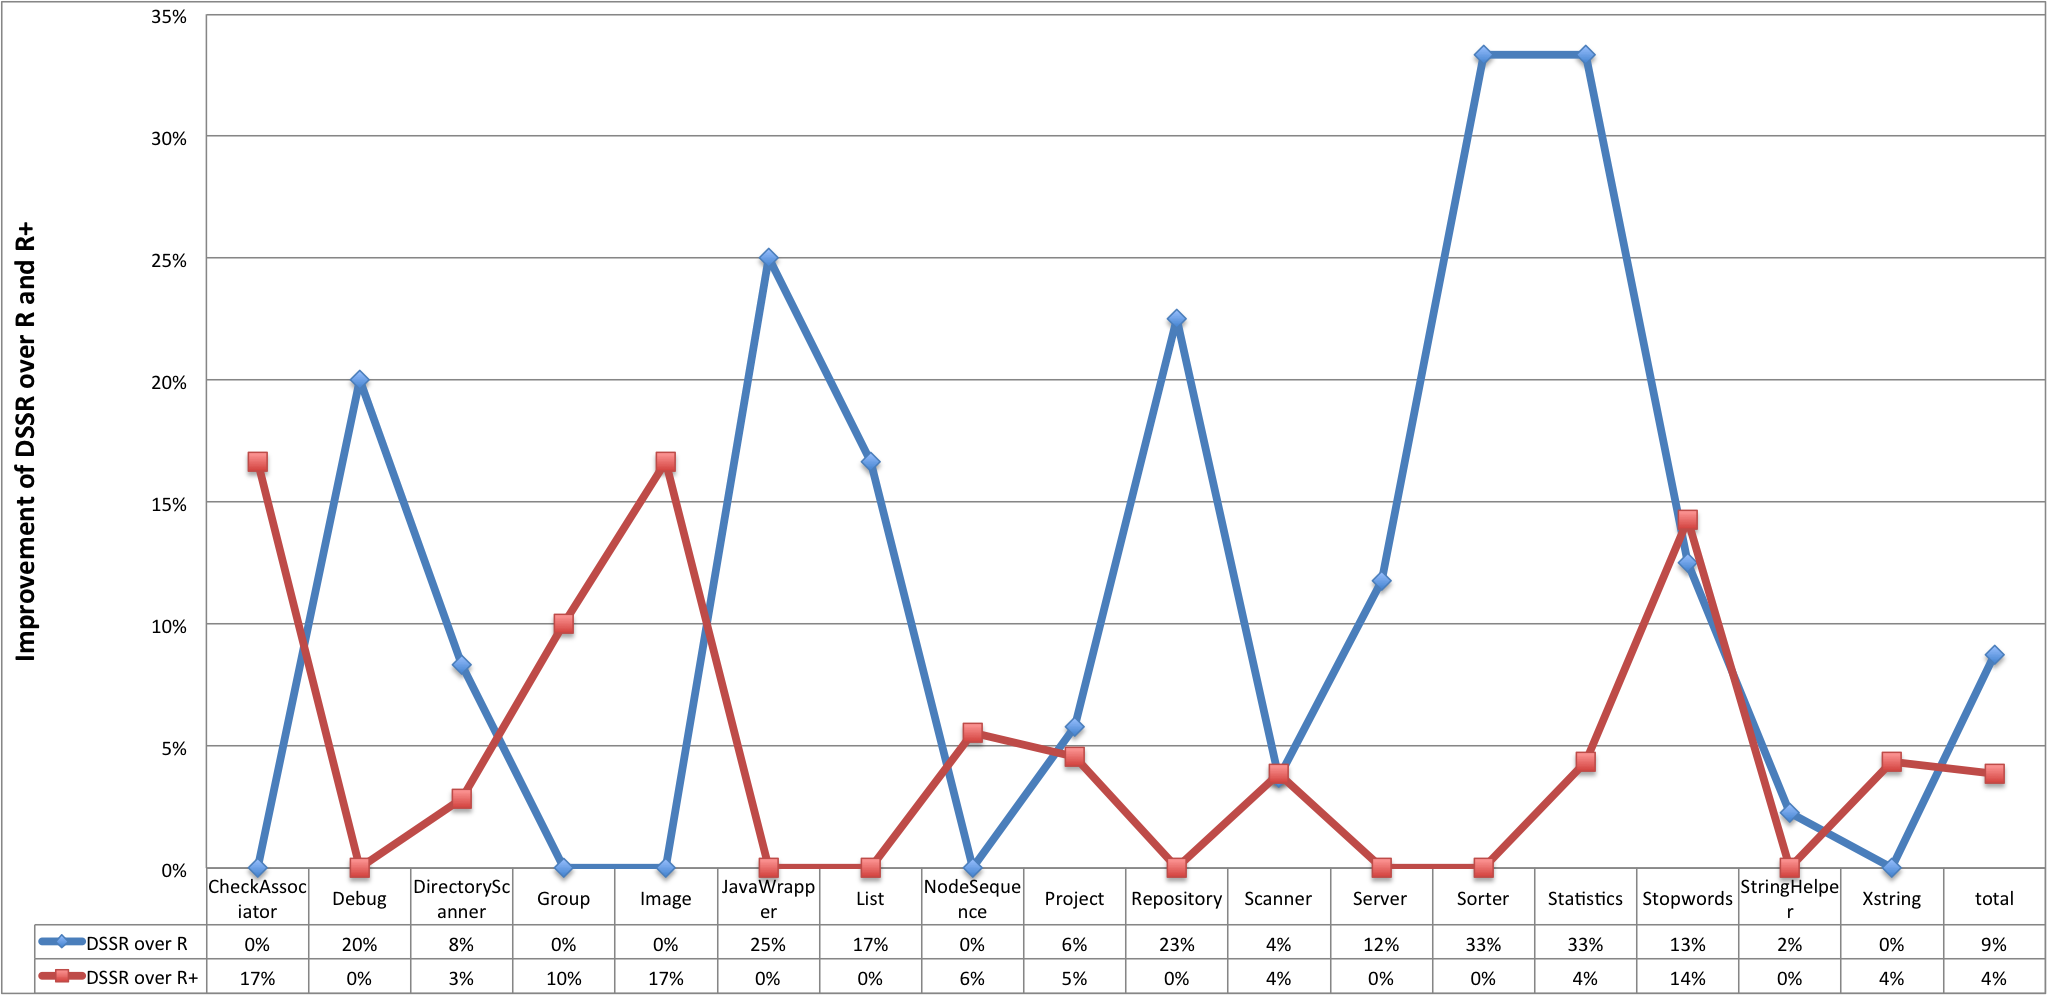
\includegraphics[width=17cm]{DSSR/DssrImprove.png}
\caption{Improvement of DSSR strategy over Random and Random+ strategy.}
\label{fig:LineChart}
\end{figure*}

%%%%%%%%%%%%%%%%%%%%%%%%%%%%%%%%%%%%%%%%%%%%



\begin{table*} [htp!]
  \scriptsize
 \caption{Complete results for R, R+ and DSSR. Results present Serial Number (S.No), Class Name, Line of Code (LOC), mean, maximum number of faults, minimum number of faults and relative standard deviation for each Random (R), Random+ (R+) and Dirt Spot Sweeping Random (DSSR) strategies.}
	%\begin{minipage}[h]{\textwidth}\centering
	\noindent\makebox[\textwidth]{
 	\begin{tabularx}{1 \textwidth}{r l r r r r r r r r r r r r r}
      %\aline
      \multirow{2}{*}{S. No}		& \multirow{2}{*}{Class Name}		& \multirow{2}{*}{LOC}	& \multicolumn{4}{c}{R}							&	\multicolumn{4}{c}{R+}							&	\multicolumn{4}{c}{DSSR}	\\
      %\cline{3-14} 
      						&						&			& Mean 	& Max	& Min 	& 	R-STD				& Mean 	& Max 	& Min 	&	 R-STD 			& Mean 		& Max 		& Min		& R-STD \\

1						& ActionTranslator			&709		& 96		&	96	&	96	& 	0					& 96		& 96 		& 96		& 		0			& 96			& 96			& 96			&	0\\     
2						& AjTypeImpl				&1180		& 80		&	83	&	79	& 	0.02					& 80		& 83 		& 79		& 		0.02			& 80			& 83			& 79			&	0.01\\      
\textbf{3}					& \textbf{Apriori}			&\textbf{292}	& \textbf{3}&	\textbf{4}	&\textbf{3}	& \textbf{0.10}			& \textbf{3}& \textbf{4} 		& \textbf{3}& \textbf{0.13}	& \textbf{3}	& \textbf{4}	& \textbf{3}	&\textbf{0.14}\\      
4						& BitSet					&575		& 9		&	9	&	9	& 	0					& 9		& 9 		& 9		& 		0			& 9			& 9			& 9			&	0\\       
5						& CatalogManager			&538		& 7		&	7	&	7	& 	0					& 7		& 7 		& 7		& 		0			& 7			& 7			& 7			&	0\\    
\textbf{6}					& \textbf{CheckAssociator}	&\textbf{351}	& \textbf{7}	&	\textbf{8}	&	\textbf{2}	& 	\textbf{0.16}					& \textbf{6}		& \textbf{9} 		& \textbf{2}		& 		\textbf{0.18}			& \textbf{7}			& \textbf{9}			& \textbf{6}			&	\textbf{0.73}\\    
\textbf{7}						& \textbf{Debug}					&\textbf{836}		& \textbf{4}		&	\textbf{6}	&	\textbf{4}	& 	\textbf{0.13}					& \textbf{5}		& \textbf{6} 		& \textbf{4}		& 		\textbf{0.12}			& \textbf{5}			& \textbf{8}			& \textbf{4}			&	\textbf{0.19}\\       
\textbf{8}						& \textbf{DirectoryScanner}			&\textbf{1714}		& \textbf{33}		&	\textbf{39}	&	\textbf{20}	& 	\textbf{0.10}					& \textbf{35}		& \textbf{38} 		& \textbf{31}		& 		\textbf{0.05}			& \textbf{36}			& \textbf{39}			& \textbf{32}			&	\textbf{0.04}\\      
9						& DiskIO					&220		& 4		&	4	&	4	& 	0					& 4		& 4 		& 4		& 		0			& 4			& 4			& 4			&	0\\      
10						& DOMParser				&92			& 7		&	7	&	3	& 	0.19					& 7		& 7 		& 3		& 		0.11			& 7			& 7			& 7			&	0\\      
11						& Entities					&328		& 3		&	3	&	3	& 	0					& 3		& 3 		& 3		& 		0			& 3			& 3			& 3			&	0\\      
12						& EntryDecoder			&675		& 8		&	9	&	7	& 	0.10					& 8		& 9 		& 7		& 		0.10			& 8			& 9			& 7			&	0.08\\   
13						& EntryComparator			&163		& 13		&	13	&	13	& 	0					& 13		& 13 		& 13		& 		0			& 13			& 13			& 13			&	0\\      
14						& Entry					&37			& 6		&	6	&	6	& 	0					& 6		& 6 		& 6		& 		0			& 6			& 6			& 6			&	0\\   
15						& Facade					&3301		& 3		&	3	&	3	& 	0					& 3		& 3 		& 3		& 		0			& 3			& 3			& 3			&	0\\   
16						& FileUtil					&83			& 1		&	1	&	1	& 	0					& 1		& 1 		& 1		& 		0			& 1			& 1			& 1			&	0\\      
17						& Font					&184		&12		&	12	&	11	& 	0.03					& 12		& 12 		& 11		& 		0.03			& 12			& 12			& 11			&	0.02\\        
18						& FPGrowth				&435		& 5		&	5	&	5	& 	0					& 5		&  5		& 5		& 		0			& 5			& 5			& 5			&	0	\\       
19						& Generator				&218		& 17		&	17	&	17	& 	0					& 17		& 17 		& 17		& 		0			& 17			& 17			& 17			&	0	\\      
\textbf{20}						& \textbf{Group}					&\textbf{88}			& \textbf{11}		&	\textbf{11}	&	\textbf{10}	& 	\textbf{0.02}					& \textbf{10}		& \textbf{4} 		& \textbf{11}		& 		\textbf{0.15}			& \textbf{11}			& \textbf{11}			& \textbf{11}			&	\textbf{0}	\\      
21						& HttpAuth				&221		& 2		&	2	&	2	& 	0					& 2		& 2 		& 2		& 		0			& 2			& 2			& 2			&	0	\\         
\textbf{22}						& \textbf{Image}					&\textbf{2146}		& \textbf{13}		&	\textbf{17}	&	\textbf{7}	& 	\textbf{0.15}					& \textbf{12}		& \textbf{14} 		& \textbf{4}	& 		\textbf{0.15}			& \textbf{14}			& \textbf{16}			& \textbf{11}			&	\textbf{0.07}\\        
23						& InstrumentTask			&71			& 2		&	2	&	1	& 	0.13					& 2		& 2 		& 1		& 		0.09			& 2			& 2			& 2			&	0	\\    
24						& IntStack					&313		& 4		&	4	&	4	& 	0					& 4		& 4 		& 4		& 		0			& 4			& 4			& 4			&	0	\\      
25						& ItemSet					&234		& 4		&	4	&	4	& 	0					& 4		& 4 		& 4		& 		0			& 4			& 4			& 4			&	0	\\       
26						& Itextpdf					&245		& 8		&	8	&	8	& 	0					& 8		&  8		& 8		& 		0			& 8			& 8			& 8			&	0\\      
\textbf{27}						& \textbf{JavaWrapper}				&\textbf{513}		&\textbf{3}		&	\textbf{2}	&	\textbf{2}	& 	\textbf{0.23}					& \textbf{4}		& \textbf{4} 		& \textbf{3}		& 		\textbf{0.06}			& \textbf{4}			& \textbf{4}			& \textbf{3}			&	\textbf{0.05}\\      
28						& JmxUtilities				&645		& 8		&	8	&	6	& 	0.07					& 8		& 8 		& 7		& 		0.04			& 8			& 8			& 7			&	0.04\\      
\textbf{29}						& \textbf{List}					&\textbf{1718}		& \textbf{5}		&	\textbf{6}	&	\textbf{4}	& 	\textbf{0.11}					& \textbf{6}		& \textbf{6} 		& \textbf{4}		& 		\textbf{0.10}			&\textbf{6}			& \textbf{6}			& \textbf{5}			&	\textbf{0.09}\\      
30						& NameEntry				&172		& 4		&	4	&	4	& 	0					& 4		& 4 		& 4		& 		0			& 4			& 4			& 4			&	0	\\  
\textbf{31}						& \textbf{NodeSequence}			&\textbf{68}			& \textbf{38}		&	\textbf{46}	&	\textbf{30}	& 	\textbf{0.10}					& \textbf{36}		& \textbf{45} 		& \textbf{30}		& 		\textbf{0.12}			& \textbf{38}			& \textbf{45}			& \textbf{30}			&	\textbf{0.08}	\\     
32						& NodeSet				&208		& 28		&	29	&	26	& 	0.03					& 28		& 29 		& 26		& 		0.04			& 28			& 29			& 26			&	0.03	\\  
33						& PersistentBag			&571		& 68		&	68	&	68	& 	0					& 68		&  68		& 68		& 		0			& 68			& 68			& 68			&	0	\\         
34						& PersistentList				&602		& 65		&	65	&	65	& 	0					& 65		&  65		& 65		& 		0			& 65			& 65			& 65			&	0	\\    
35						& PersistentSet				&162		& 36		&	36	&	36	& 	0					& 36		&  36		& 36		& 		0			& 36			& 36			& 36 			&	0	\\        
\textbf{36}						& \textbf{Project}					&\textbf{470}		& \textbf{65}		&	\textbf{71}	&	\textbf{60}	& 	\textbf{0.04}					& \textbf{66}		&  \textbf{78}		& \textbf{62}		& 		\textbf{0.04}			& \textbf{69}			& \textbf{78}			& \textbf{64}			&	\textbf{0.05}	\\        
\textbf{37}						& \textbf{Repository}				&\textbf{63}			& \textbf{31}		&	\textbf{31}	&	\textbf{31}	& 	\textbf{0}					& \textbf{40}		&  \textbf{40}		& \textbf{40}		& 		\textbf{0}			& \textbf{40}			& \textbf{40}			& \textbf{40}			&	\textbf{0}	\\         
38						& Routine					&1069		& 7		&	7	&	7	& 	0					& 7		&  7		& 7		& 		0			& 7			& 7			& 7			&	0	\\
39						& RubyBigDecimal			&1564		& 4 		&	4	&	4	& 	0					& 4		& 4 		& 4		& 		0			& 4			& 4			& 4			&	0\\      
40						& Scanner				&94			& 3		&	5	&	2	& 	0.20					& 3		& 5 		& 2		& 		0.27			& 3			& 5			& 2			&	0.25\\      
\textbf{41}						& \textbf{Scene}					&\textbf{1603}		& \textbf{26}		&	\textbf{27}	&	\textbf{26}	& 	\textbf{0.02}					& \textbf{26}		& \textbf{27} 		& \textbf{26}		& 		\textbf{0.02}			& \textbf{27}			& \textbf{27}			& \textbf{26}			&	\textbf{0.01}\\      
42						& SelectionManager			&431		& 3		&	3	&	3	& 	0					& 3		& 3 		& 3		& 		0			& 3			& 3			& 3			&	0\\      
\textbf{43}						& \textbf{Server}					&\textbf{279}		&\textbf{15}		&	\textbf{21}	&	\textbf{11}	& 	\textbf{0.20}					& \textbf{17}		& \textbf{21} 		& \textbf{12}		& 		\textbf{0.16}			& \textbf{17}			& \textbf{21}			& \textbf{12}			&	\textbf{0.14}\\      
\textbf{44}						& \textbf{Sorter}					&\textbf{47}			& \textbf{2}		&	\textbf{2}	&	\textbf{1}	& 	\textbf{0.09}					& \textbf{3}		& \textbf{3} 		& \textbf{2}		& 		\textbf{0.06}			&\textbf{3}			& \textbf{3}			& \textbf{3}			&	\textbf{0}\\      
45						& Sorting					&762		& 3		&	3	&	3	& 	0					& 3		& 3 		& 3		& 		0			& 3			& 3			& 3			&	0\\      
\textbf{46}						& \textbf{Statistics}				&\textbf{491}		& \textbf{16}		&	\textbf{17}	&	\textbf{12}	&	\textbf{0.08}					& \textbf{23}		& \textbf{25} 		& \textbf{22}		& 		\textbf{0.03}			& \textbf{24}			& \textbf{25}			& \textbf{22}			&	\textbf{0.04}\\      
47						& Status					&32			& 53		&	53	&	53	& 	0					& 53		& 53 		& 53		& 		0			& 53			& 53			& 53			&	0\\      
\textbf{48}						& \textbf{Stopwords}				&\textbf{332}		& \textbf{7}		&	\textbf{8}	&	\textbf{7}	& 	\textbf{0.03}					& \textbf{7}		&  \textbf{8}		& \textbf{6}		& 		\textbf{0.08}			& \textbf{8}			& \textbf{8}			& \textbf{7}			&	\textbf{0.06}\\      
\textbf{49}						& \textbf{StringHelper}				&\textbf{178}		& \textbf{43}	 	& 	\textbf{45}	&	\textbf{40}	& 	\textbf{0.02}					& \textbf{44}		&  \textbf{46}		& \textbf{42}		& 		\textbf{0.02}			& \textbf{44}			& \textbf{45}			& \textbf{42}			&	\textbf{0.02}\\      
50						& StringUtils				&119		& 19 		&	19	&	19	& 	0					& 19		& 19 		& 19		& 		0			& 19			& 19			& 19			&	0\\      
51						& TouchCollector			&222		& 3		&	3	&	3	& 	0					& 3		&  3		& 3		& 		0			& 3			& 3			& 3			&	0\\      
52						& Trie					&460		& 21		&	22	&	21	& 	0.02					& 21		&  22		& 21		& 		0.01			& 21			& 22			& 21			&	0.01\\      
53						& URI					&3970		& 5 		&	5	&	5	& 	0					& 5		&  5		& 5		& 		0			& 5			& 5			& 5			&	0\\      
54						& WebMacro				&311		& 5		&	5	&	5	& 	0					& 5		&  6		& 5		& 		0.14			& 5			& 7			& 5			&	0.28\\      
55						& XMLAttributesImpl			&277		& 8		&	8	&	8	& 	0					& 8		&  8		& 8		& 		0			& 8			& 8			& 8			&	0\\      
56						& XMLChar				&1031		& 13		&	13	&	13	& 	0					& 13		&  13		& 13		& 		0			& 13			& 13			& 13			&	0\\      
57						& XMLEntityManger			&763		& 17		&	18	&	17	& 	0.01					& 17		&  17		& 16		& 		0.01			& 17			& 17			& 17			&	0\\      
58						& XMLEntityScanner			&445		& 12		&	12	&	12	& 	0					& 12		&  12		& 12		& 		0			& 12			& 12			& 12			&	0\\      
59						& XObject					&318		& 19		&	19	&	19	& 	0					& 19		&  19		& 19		& 		0			& 19			& 19			& 19			&	0\\      
\textbf{60}						& \textbf{XString}					&\textbf{546}		& \textbf{23}		&	\textbf{24}	&	\textbf{21}	& 	\textbf{0.04}					& \textbf{23}		&  \textbf{24}		& \textbf{23}		& 		\textbf{0.02}			& \textbf{24}			& \textbf{24}			& \textbf{23}			&	\textbf{0.02}\\      

    						\multicolumn{2}{c}{\textbf{Total}}	&35,785	&1040	&	1075	&    973	&	2.42				& 1061	&1106	&1009	&		2.35		& 1075		& 1118		& 1032		& 	1.82\\
   %\hline
     \end{tabularx} }
 	%\end{minipage}
    \bigskip
    \label{table:Results}
\end{table*}

\section{Results}\label{sec:res}
Results of the experiments including class name, Line of Code (LOC), mean value, maximum and minimum number of unique failures and relative standard deviation for each of the 60 classes tested using R, R+ and DSSR strategy are presented in Table~\ref{table:Results}. Each strategy found an equal number of faults in 31 classes while in the remaining 29 classes the three strategies performed differently from one another. The total of mean values of unique failures in DSSR (1075) is higher than for R (1040) or R+ (1061) strategies. 
%Results given in Table~\ref{table:ttest} can be split into three different categories as shown in Table~\ref{table:categories}. 
DSSR also finds a higher number of maximum unique failures (1118) than both R (1075), and R+ (1106). DSSR strategy finds 43 and 12 more unique faults compared to R and R+ respectively. The minimum number of unique faults found by DSSR (1032) is also higher than for R (973) and R+ (1009) which attributes to higher efficiency of DSSR strategy over R and R+ strategies. 

% How to write relative standard deviation.
% Eventually, the standard deviations are all of the order of magnitude of .1\% for all strategies.

\subsection{Is there an absolute best among R, R+ and DSSR strategies?}
Based on our findings DSSR is at least as good as R and R+ in almost all cases, it is also significantly better than both R and R+ in 12\% of the classes. Figure~\ref{fig:LineChart} presents the average improvements of DSSR strategy over R and R+ strategy over the 17 classes for which there is a significant difference between DSSR and R or R+. The blue line with diamond symbol shows performance of DSSR over R and the red line with square symbols depicts the improvement of DSSR over R+ strategy. The classes where blue line with diamond symbols show the improvement of DSSR over R and red line with square symbols show the improvement of DSSR over R+. 

The improvement of DSSR over R and R+ strategy is calculated by applying the formula (1) and (2) respectively.

\begin{equation} \frac{Averagefaults_{(DSSR)} - Averagefaults_{(R)}}{Averagefaults_{(R)}} * 100  \end{equation}

\begin{equation} \frac{Averagefaults_{(DSSR)} - Averagefaults_{(R+)}}{Averagefaults_{(R+)}}  * 100 \end{equation}

The findings show that DSSR strategy perform up to 33\% better than R and up to 17\% better than R+ strategy. In some cases DSSR perform equally well with R and R+ but in no case DSSR performed lower than R and R+. Based on the results it can be stated that DSSR strategy is a better choice than R and R+ strategy. 



\begin{table*}[htp]
\small
\caption{T-test results of the classes showing different results}
\centering
\begin{tabular}{rlrrrl}
 \multirow{2}{*} {S. No}	& \multirow{2}{*}{Class Name}	&  \multicolumn{3}{c}{T-test Results} & \multirow{2}{*}{Interpretation} \\

								& & 	DSSR, R	& DSSR, R+	&  R, R+ 	& 		\\

1		&	AjTypeImpl		&	1 				& 1 			& 1			& 		\\	
2		&	Apriori			&	\textbf{0.03}	 	& 0.49		& 0.16		&		\\	
3		&	CheckAssociator	&	\textbf{0.04}	 	& \textbf{0.05}	& 0.44		& DSSR better		\\	
4		&	Debug			&	\textbf{0.03}	 	& 0.14		& 0.56		&		\\	
5		&	DirectoryScanner	&	\textbf{0.04}	 	& \textbf{0.01}	& 0.43		& DSSR better		\\
6		&	DomParser		&	\textbf{0.05}	 	& 0.23		& 0.13		&				\\
7		&	EntityDecoder		&	\textbf{0.04}	 	& 0.28		& 0.3			&		\\			
8		&	Font				&	0.18	 			& 0.18		& 1			&		\\
9		&	Group			&	0.33	 			& \textbf{0.03}	& \textbf{0.04}	& DSSR = R > R+	\\
10		&	Image			&	\textbf{0.03}		& \textbf{0.01}	& 0.61		& DSSR better \\		
11		&	InstrumentTask		&	0.16				& 0.33		& 0.57		& \\
12		&	JavaWrapper		&	\textbf{0.001}		& 0.57		& 0.004		& DSSR = R+ > R \\
13		& 	JmxUtilities		&	0.13				& 0.71		& 0.08		&	\\
14		&	List				& 	\textbf{0.01}		&0.25		&\textbf{0}		& DSSR = R+ > R \\
15		&	NodeSequence	&	0.97				&\textbf{0.04}	&\textbf{0.06}	& DSSR = R > R+ \\
16		&	NodeSet			&	\textbf{0.03}		&0.42		&0.26		& 	\\
17		&	Project			&	\textbf{0.001}		&0.57		&\textbf{0.004}	& DSSR better \\		
18		&	Repository		&	\textbf{0}			&1			&\textbf{0}		& DSSR = R+ > R \\
19		&	Scanner			&	1				&\textbf{0.03}	&\textbf{0.01}	& DSSR better \\
20		&	Scene			&	\textbf{0}			&\textbf{0}		& 1			& DSSR better \\
21		&	Server			&	\textbf{0.03}		& 0.88		&\textbf{0.03} 	& DSSR = R+ > R \\
22		&	Sorter			& 	\textbf{0}			& 0.33		&\textbf{0}		& DSSR = R+ > R \\
23		&	Statistics			&	\textbf{0}			& 0.43		&\textbf{0}		& DSSR = R+ > R\\
24		&	Stopwords		&	\textbf{0}			& 0.23		&\textbf{0}		& DSSR = R+ > R \\
25		&	StringHelper		&	\textbf{0.03}		& 0.44		&0.44		& DSSR = R+ > R\\
26		& 	Trie				&	0.1				& 0.33		&0.47		& DSSR better \\
27		&	WebMacro		&	0.33				& 1			&0.16		& \\
28		&	XMLEntityManager	&	0.33				& 0.33		&0.16		& \\
29 		&	XString			&	0.14				&\textbf{0.03}	&0.86		& \\


\end{tabular}
\bigskip
\label{table:ttest}
\end{table*}





\subsection{Are there classes for which any of the three strategies provide better results?}


T-tests applied to the data given in Table~\ref{table:ttest} show that DSSR is significantly better in 7 classes from R and R+ strategy, in 8 classes DSSR performed similarly to R+  but significantly higher than R, and in 2 classes DSSR performed similarly to R but significantly higher than R+. There is no case R and R+ strategy performed significantly better than DSSR strategy. Expressed in percentage: 72\%  of the classes do not show significantly different behaviours whereas in 28\% of hte classes, the DSSR strategy performs significantly better than at least one of R and R+. It is interesting to note that in no single case R and R+ strategies performed better than DSSR strategy. We attribute this to DSSR possessing the qualities of R and R+ whereas containing the spot sweeping feature.


%Results of the 60 classes tested in the study are divided in to 11 different categories as presented in ~\ref{table:categories}. 
\begin{comment}
\begin{table}[h]
\caption{Results of the 60 classes are divided into 11 categories}
\centering
\begin{tabular}{|r|l|r|}
\hline
S. No	& 	Category			& 	Result\\
\hline
1		&	DSSR > R			&	12 \\	
2		&	DSSR > R+		&	10 \\	
3		&	DSSR = R			&	5 \\	
4		&	DSSR = R+		&	7 \\	
5		&	R+ > R 			&	10 \\	
6		&	R+ < R			&	5 \\	
7		&	R+ = R			&	2 \\	
8		&	R > R+			&	4 \\
9		&	DSSR < R			&	0 \\	
10		&	DSSR < R+		&	0 \\
11		&	DSSR = R = R+	&	43 \\			
\hline
\end{tabular}
\bigskip
\label{table:categories}
\end{table}

% pie chart is removed because the length of the paper is exceeding 10 pages and also it don't make much sense i believe.
%\begin{figure}[h]
%\centering
%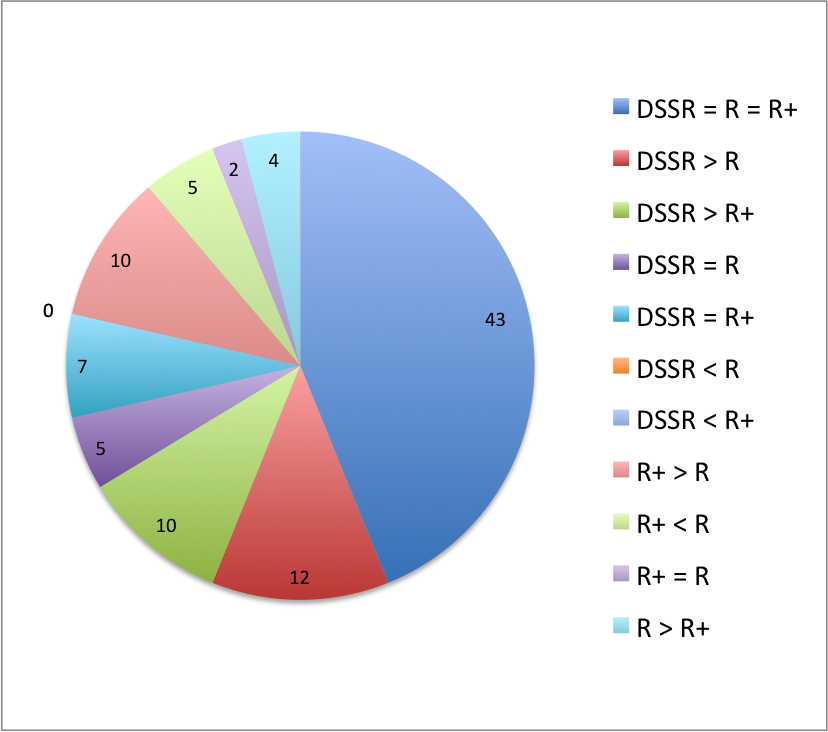
\includegraphics[width=8cm,height=7cm]{pie5.png}
%\caption{Division of result in to categories}
%\label{fig:pie}
%\end{figure}






The first category contain 12 classes where DSSR strategy performs better than R. 
The second category contain 10 classes where DSSR strategy performs better than R+. 
The third category contain 5 classes where DSSR strategy and R performs equally well.
The fourth category contain 7 classes where DSSR and R+ performs equally well. 
The fifth category contain 10 classes where R+ performs better than R.
The sixth category contain 5 classes where R performs better than R+.
The seventh category contain 2 classes where R and R+ performs equally well.
The eighth category contain 4 classes where R performs better than R+.
Category 9 and 10 shows that neither R nor R+ performed better than DSSR strategy.
The last category shows each strategy performing equally well for 43 classes. Expressing in percentage, 72\% classes do not show different behaviours whereas in 28\% of classes, the DSSR strategy performs better than R and R+ strategy. It is interesting to note that in no single case R and R+ strategies performed better than DSSR strategy. This is attributed to the fact that DSSR strategy possess the qualities of R and R+ and has the additional advantage of spot sweeping.

\end{comment}

\subsection{Can we pick the best default strategy between R, R+ and DSSR?}

Analysis of the experimental data reveal that DSSR strategy has an edge over R and R+. This is because of the additional feature of Spot Sweeping in DSSR strategy.

In spite of the better performance of DSSR strategy compared to R and R+ strategies the present study does not provide ample evidence to pick it as the best default strategy because of the overhead induced by this strategy (see next section). Further study might give conclusive evidence. 




%%%%%%%%%%%%%%%%%    DISCUSSION   %%%%%%%%%%%%%%%%%%%%

\section{Discussion}\label{sec:discussion}
In this section we discuss various factors such as the time taken, effect of test duration, number of tests, number of faults in the different strategies and the effect of finding first fault in the DSSR strategy.
\textbf{Time taken to execute an equal number of test cases:}
The DSSR strategy takes slightly more time (up to 5\%) than both pure random and random plus which may be due to maintaining sets of interesting values during the execution. We do not believe that the overhead can be reduced. 

\textbf{Effect of test duration and number of tests on the results:}
All three techniques have the same potential for finding failures. If testing is continued for a long duration then all three strategies will find the same number of unique failures and the results will converge. We suspect however that some of the unique failures will take an extremely long time to be found by using random or random+ only. Further experiments should confirm this point.


\textbf{Effect of number of faults on results:} 
We found that the DSSR strategy performs better when the number of faults is higher in the code. The reason seems to be that when there are more faults, their domains are more connected and DSSR strategy works better. Further studies might use historical data to pick the best strategy.

\textbf{Dependence of DSSR strategy to find the first unique failure early enough:}
During the experiments we noticed that if a unique failure is not found  quickly enough, there is no value added to the list of interesting values and then the test becomes equivalent to random+ testing. This means that better ways of populating failure-inducing values are needed for sufficient leverage to DSSR strategy. As an example, the following piece of code would be unlikely to fail under the current setting:

\begin{lstlisting}
public void test(float value){
 if(value == 34.4445)   10/0;
}
\end{lstlisting}

In this case, we could add constant literals from the SUT to the list of interesting values in a dynamic fashion. These literals can be obtained from the constant pool in the class files of the SUT.

In the example above the value 34.4445 and its surrounding values would  be added to the list of interesting values before the test starts and the DSSR strategy would find the unique failure right away.

\textbf{DSSR strategy and coverage:} Random strategies typically achieve high level of coverage~\cite{Oriol2010}. It might also be interesting to compare R, R+ and DSSR with respect to the achieved coverage or even to use a DSSR variant that adds a new interesting value and its neighbours when a new branch is reached.


\textbf{Threats to validity:} As usual with such empirical studies, the present work might suffer from a non-representative selection of classes.
The selection in the current study is however made through random process and objective criteria, therefore, it seems likely that it would be representative.

The parameters of the study might also have prompted incorrect results. But this is unlikely due to previous results on random testing~\cite{Oriol2012}.



%%%%%%%%%%%%%%%%%    RW   %%%%%%%%%%%%%%%%%%%%

\section{Related Work}\label{sec:rw}

Random testing is a popular technique with simple algorithm but proven to find subtle faults in complex programs and Java libraries~\cite{Pacheco2005, Csallner2004, Claessen2000a}. Its simplicity, ease of implementation and efficiency in generating test cases make it the best choice for test automation~\cite{Hamlet1994}. Some of the well known automated tools based on random strategy includes Jartege~\cite{Oriat2004}, Eclat~\cite{Pacheco2005}, JCrasher~\cite{Csallner2004}, AutoTest \cite{Ciupa2007, Ciupa2008a} and YETI~\cite{Oriol2010, Oriol2012}.

In pursuit of better test results and lower overhead, many variations of random strategy have been proposed~\cite{Chen2010, Chen2005, Chan2002, Chen2004a, Chen2003}. Adaptive random testing (ART), Quasi-random testing (QRT) and Restricted Random testing (RRT) achieved better results by selecting test inputs randomly but evenly spread across the input domain. Mirror ART and ART through dynamic partitioning increased the performance by reducing the overhead of ART. The main reason behind better performance of the strategies is that even spread of test input increases the chance of exploring the fault patterns present in the input domain.

A more recent research study \cite{Yoo2012} stresses on the effectiveness of data regeneration in close vicinity of the existing test data. Their findings showed up to two orders of magnitude more efficient test data generation than the existing techniques. Two major limitations of their study are the requirement of existing test cases to regenerate new test cases, and increased overhead due to ``meta heuristics search'' based on hill climbing algorithm to regenerate new data. In DSSR no pre-existing test cases are required because it utilises the border values from R+ and regenerate the data very cheaply in a dynamic fashion different for each class under test without any prior test data and with comparatively lower overhead. 
  
The random+ (R+) strategy is an extension of the random strategy in which interesting values, beside pure random values, are added to the list of test inputs~\cite{Leitner2007}. These interesting values includes border values which have high tendency of finding faults in the given SUT~\cite{Beizer1990}. Results obtained with R+ strategy show significant improvement over random strategy~\cite{Leitner2007}. DSSR strategy is an extension of R+ strategy which starts testing as R+ until a fault is found then it switches to spot sweeping.

%It is interesting that numerous efforts have been made to discover the fault patterns~\cite{Chen2010, Chen2005, Chan2002, Chen2004a, Chen2003}, etc. but in our knowledge, none has been published on covering/sweeping all the faults lying in a specific pattern once it has been discovered.


A common practice to evaluate performance of an extended strategy is to compare the results obtained by applying the new and existing strategy to identical programs~\cite{Gutjahr1999, Duran1984, Hamlet1990}. Arcuri et al. \cite{Arcuri2012}, stress on the use of random testing as a baseline for comparison with other test strategies. We followed the procedure and evaluated DSSR strategy against R and R+ strategies under identical conditions.

In our experiments we selected projects from the Qualitas Corpus~\cite{Tempero2010} which is a collection of open source java programs maintained for independent empirical research. The projects in Qualitas Corpus are carefully selected that spans across the whole set of java applications~\cite{Oriol2012, Tempero2010a, Tempero2008}.


%%%%%%%%%%%%%%%%%    CONCLUSIONS   %%%%%%%%%%%%%%%%%%%%


\section{Conclusions}\label{sec:conc}
The main goal of the present study was to develop a new random strategy which could find more faults in lower number of test cases. We developed a new strategy named. ``DSSR strategy'' as an extension of R+, based on the assumption that in a significant number of classes, failure domains are contiguous or located closely. The DSS strategy, a strategy which adds neighbouring values of the failure finding value to a list of interesting values, was implemented in the random testing tool YETI to test 60 classes, 30 times each, from Qualitas Corpus with each of the 3 strategies R, R+ and DSSR. The newly developed DSSR strategy uncovers more unique failures than both random and random+ strategies with a 5\% overhead. We found out that for 7 (12\%) classes DSSR was significantly better than both R+ and R, for 8 (13\%) classes DSSR performed similarly to R+ and significantly better than R, while in 2 (3\%) cases DSSR performed similarly to R and significantly better than R+. In all other cases, DSSR, R+ and R do not seem to perform significantly differently. Overall, DSSR yields encouraging results and advocates to develop the technique further for settings in which it is significantly better than both R and R+ strategies.
}%{\input{TwoAbstractionsInCMAC}}

%% The chapter on the Reward Shaping Analysis in model-free RL
%\ychapter{Extraction of Multilingual Synsets from Aligned
%Corpora}{Extraction of Multilingual Synsets from Aligned
%Corpora\label{CHAP:RSANALYSIS}}{\input{Rshaping_Analysis}}

\ychapter{Automated Discovery of Failure Domain Strategy}{Automated Discovery of Failure Domain Strategy\label{CHAP:ADFD}}{

\section{Introduction}\label{sec:intro}

Testing is fundamental requirement to assess the quality of any software. Manual testing is labour-intensive and error-prone; therefore emphasis is to use automated testing that significantly reduces the cost of software development process and its maintenance \cite{Beizer1995}. Most of the modern black-box testing techniques execute the System Under Test (SUT) with specific input and compare the obtained results against the test oracle. A report is generated at the end of each test session containing any discovered faults and the input values which triggers the faults. Debuggers fix the discovered faults in the SUT with the help of these reports. The revised version of the system is given back to the testers to find more faults and this process continues till the desired level of quality, set in test plan, is achieved.

The fact that exhaustive testing for any non-trivial program is impossible, compels the testers to come up with some strategy of input selection from the whole input domain. Pure random is one of the possible strategies widely used in automated tools. It is intuitively simple and easy to implement \cite{Ciupa2008},  \cite{Forrester2000}. It involves minimum or no overhead in input selection and lacks human bias \cite{Hamlet1994},  \cite{Linger1993}. While pure random testing has many benefits, there are some limitations as well, including low code coverage \cite{Offutt1996} and discovery of lower number of faults \cite{Chen1994}. To overcome these limitations while keeping its benefits intact many researchers successfully refined pure random testing. Adaptive Random Testing (ART) is the most significant refinements of random testing. Experiments performed using ART showed up to 50\% better results compared to the traditional/pure random testing  \cite{Chen2008}.  Similarly Restricted Random Testing (RRT) \cite{Chan2002}, Mirror Adaptive Random Testing (MART)  \cite{Chen2004}, Adaptive Random Testing for Object Oriented Programs (ARTOO) \cite{Ciupa2008}, Directed Adaptive Random Testing (DART)  \cite{Godefroid2005}, Lattice-based Adaptive Random Testing (LART) \cite{Mayer2005} and Feedback-directed Random Testing (FRT) \cite{Pacheco2007} are some of the variations of random testing aiming to increase the overall performance of pure random testing.

All the above-mentioned variations in random testing are based on the observation of Chan et. al.,  \cite{Chan1996} that failure causing inputs across the whole input domain form certain kinds of domains. They classified these domains into point, block and strip fault domain. In Figure \ref{fig:patterns} the square box represents the whole input domain. The black point, block and strip area inside the box represent the faulty values while white area inside the box represent legitimate values for a specific system. They further suggested that the fault finding ability of testing could be improved by taking into consideration these failure domains.

\begin{figure}[h]
 \centering
\includegraphics[width=8cm,height=2cm]{ADFD/ART_Patterns.png}
\caption{Failure domains across input domain \cite{Chan1996}}
\label{fig:patterns}
\end{figure}


% It is important to note that these techniques only identify a single instance of failure and do not  focus on the failure domain. 

%2.	It is also noticed that further analysis of fault lead to new faults which the testing process may not have identified.
%3. 	Experiments can be performed to analyse the frequency of existence of point, block and strip domain across the input domain. 

%Random testing is a black-box testing technique in which parts (methods/modules) of SUT are selected randomly and then executed against randomly generated test data from the whole input domain. Results obtained from the execution are either compared to the specifications of the SUT or language exceptions which served as a test oracle. Any test output that fail to meet the oracle either because of failing to comply the specification or trigger the exceptions are considered as potential faults. In this paper we present a new tool, called Automated Discovery of Failure Domain (ADFD), based on a random testing tool called York Extensible Testing Infrastructure (YETI), for not only finding fault but also its domain. ADFD utilise YETI to discover the fault in the given SUT and then generate a dynamic code for finding its domain. The found domain -- point, block or strip are presented on the graph at the end of each test session


%ADFD has been designed to decrease the time of system testing. Knowing the domain of the fault the debuggers This research can decrease the overall testing time by reducing the number of code exchanges between testers and debugger. It is achieved by tracking the failure domain and not only a single instance failure. Tracking failure domain provide more information about the behaviour of the fault.

%that also served as regression testing. None of the testing techniques evaluate the nature of the fault and the pattern in which the fault reside. 


%The aim of this research study is to find not only find the values for which the system fails but also the domains of failure causing inputs which will help in automated generation of fault targeted test cases for any black-box testing technique.\\


%Over the past few years there is a tremendous growth in development of hardware whose main focus is to increase the computer processing power. The computers that served as a mini and mainframe computers few years ago are turned into personal computer in todays modern age. To utilise this processing power various software development companies started to develop more sophisticated and processing hungry softwares. These softwares provide simple and easy to use Graphical User Interface (GUI) but on the back end they are equally complex and consist of thousands of instructions. This increase in size of the software also increases the difficulty of preserving high quality, reliability, portability, maintainability and efficiency of the software. These problems are mainly cater by software testing. The increase of complexity and size of softwares also forced the researchers to find new ways of software testing that are more efficient, reliable and speedy to cope with the ever increasing hardware and software industry.\\

%Mirror Adaptive Random Testing (MART)  \cite{Chen2003}, Feedback-directed Random Testing (FDRT) \cite{Pacheco2007}, Restricted Random Testing (RRT) \cite{Chan2002} and Quasi Random Testing  (QRT) \cite{Chen2005} are the strategies based on the same principle that found better results compared to ordinary random testing.

It is interesting that where many random strategies are based on the principle of contiguous fault domains inside the input domain, no specific strategy is developed to evaluate these fault domains. This paper describes a new test strategy called Automated Discovery of Failure Domain (ADFD), which not only finds the pass and fail input values but also finds their domains. The idea of identification of pass and fail domain is attractive as it provides an insight of the domains in the given SUT. Some important aspects of ADFD strategy presented in the paper include:

\begin{itemize}
\item Implementation of the new ADFD strategy in York Extensible Testing Infrastructure (YETI) tool.
\item Evaluation to assess ADFD strategy by testing classes with different fault domains.
\item Decrease in overall test duration by identification of all the fault domains instead of a single instance of fault.
\item Increase in test efficiency by helping debugger to keep in view all the fault occurrences when debugging. 
\end{itemize}


% Additionally, ADFD test strategy can also be used to identify frequency of point, block and strip fault domain across the production softwares.



%The main objective behind ADFD is to get an automated frame work that find the existence of fault and fault domain across the input domain, decrease debugging time and to discover any more faults missed by the testing system. Significant research has been done to utilise the failure domains but their existence, nature and boundaries need further attention. Having fault domain information prior to testing enables the tester to guide testing according to the failure domain of the SUT, for example pure random testing is more effective for point domain than block and strip domains where as ART, MART, FDRT, RRT and QRT are more effective for block and strip fault domains than point fault domain.

%In our previous research we extended the same idea of the existence of different domains of failure across the whole input domain proposed by Chen et al, \cite{Chen2008} and accepted by various other researchers to develop a new strategy called Dirt Spot Sweeping Strategy [X]. However the experimental results showed not very considerable improvement then what we predicted. We performed 500 experiments in which we carried out 10000 tests but the results showed only 5\% improvement contrary to our prediction of 30\%. All the experiments were performed from a pool of open-source projects bundled in a repository called Qualitas Corpus \cite{Tempero2010}. Corpus contains more than 100 open-source java projects and maintained only for the purpose of unbiased research experiments. Therefore one of the conclusions derived from our experiments was that the patterns of failure may not exist in most of the software’s due to which our strategy which focus on these patterns didn’t produce much efficiency.\\
%It was therefore very interesting for us to do further research to find about the existence and nature of these failure patterns. Our main focus in this research paper is to discover whether there exist failure patterns across the input domain or not and if they exist then how frequent and what pattern they follow.\\

The rest of this paper is organized as follows: \\ Section~\ref{sec:adfd} describes the ADFD strategy. Section~\ref{sec:implementation} presents implementation of the ADFD strategy. Section~\ref{sec:experimentalResults} explains the experimental results. Section~\ref{sec:discussion} discusses the results. Section~\ref{sec:validity} presents the threats to validity. Section~\ref{sec:relatedWork} presents related work and Section~\ref{sec:conclusion}, concludes the study.

%In Section II, we describe the automated discovery of failure domain test strategy and explain its structure and function with the help of a flowchart and motivating example. Section III presents its implementation in automated random testing tool called York Extensible Testing Infrastructure (YETI). Section IV and V report the experiments performed using the proposed technique and evaluate \& discuss the obtained results. Section VI and VII discuss any threats to validity and related discussion. Finally we conclude in Section VIII. 

%The rest of this paper is organized as follows. The sections, II to X, describe automated strategy, Implementation, Experimental setup and analysis, Evaluation, Experimental results, discussion, conclusion and future work respectively.\\

%X\section{Problems and Solutions}\label{sec:probl_and_sol}
%This paper address five. main problems in random testing. These are (1) Finding the whole domain of fault instead of only failing values, (2) Representation of fault values, (3) automation of the evaluation process, (4) Identification of fault domain for multi arguments methods and its representation, (5) Generation and classification of test values for Strings and complex (non scaler) arguments. This section elaborate each of the above mention problem and describe our proposed solution (if any) to them.

%\subsection{Finding the whole domain of fault instead of only failing values}
%Most of the testing tools take into account only the fault finding values with out giving due consideration to the domain in which the values exist. \subsection{Representation of fault values and fault domains}
%points: instead of dumping logs and more complex reports we describe the fault domains with the help of charts. 
%\subsection{Automation of the testing process}
%We developed an automated system to test the system, generate the fault domain finding files, compile and execute them to find the fault domains if any. points: automation is achieved by combining the test tool and evaluation system e.g. yeti and ADFD.   
%\subsection{Identification and representation of multi arguments data}
%I think it is beyond the scope of this study to identify and represent more then 3 arguments method because at the moment we can show only three diminutional charts.
%\subsection{Generation and classification of test values for string and complex (non scaler) arguments}
%It is difficult to find the domain for strings and complex (non scaler) data therefore they can be exempted from this study.


\section{Automated Discovery of Failure Domain}\label{sec:adfd}

Automated Discovery of Failure Domain (ADFD) strategy is proposed as improvement on R+ strategy with capability of finding faults as well as the fault domains. The output produced at the end of test session is a chart showing the passing value or range of values in green and failing value or range of values in red. The complete workflow of ADFD strategy is given in Figure \ref{fig:ADFD}.

The process is divided into five major steps given below and each step is briefly explained in the following paras.

\begin{enumerate}
\item GUI front-end for providing input
\item Automated finding of fault
\item Automated generation of modules
\item Automated compilation and execution of modules to discover domains
\item Automated generation of graph showing domains
\end{enumerate}

\begin{figure}[ht]
\centering
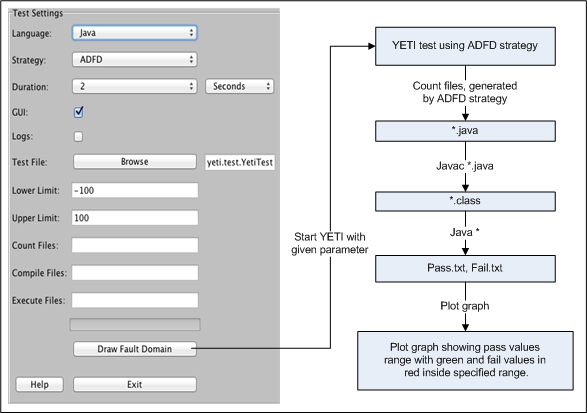
\includegraphics[width=8.2cm,height=6cm]{ADFD/ADFD-Diagram1.png}
\caption{Work flow of ADFD strategy}
\label{fig:ADFD}
\end{figure}

\begin{figure}[htp]
\begin{center}
%\centring
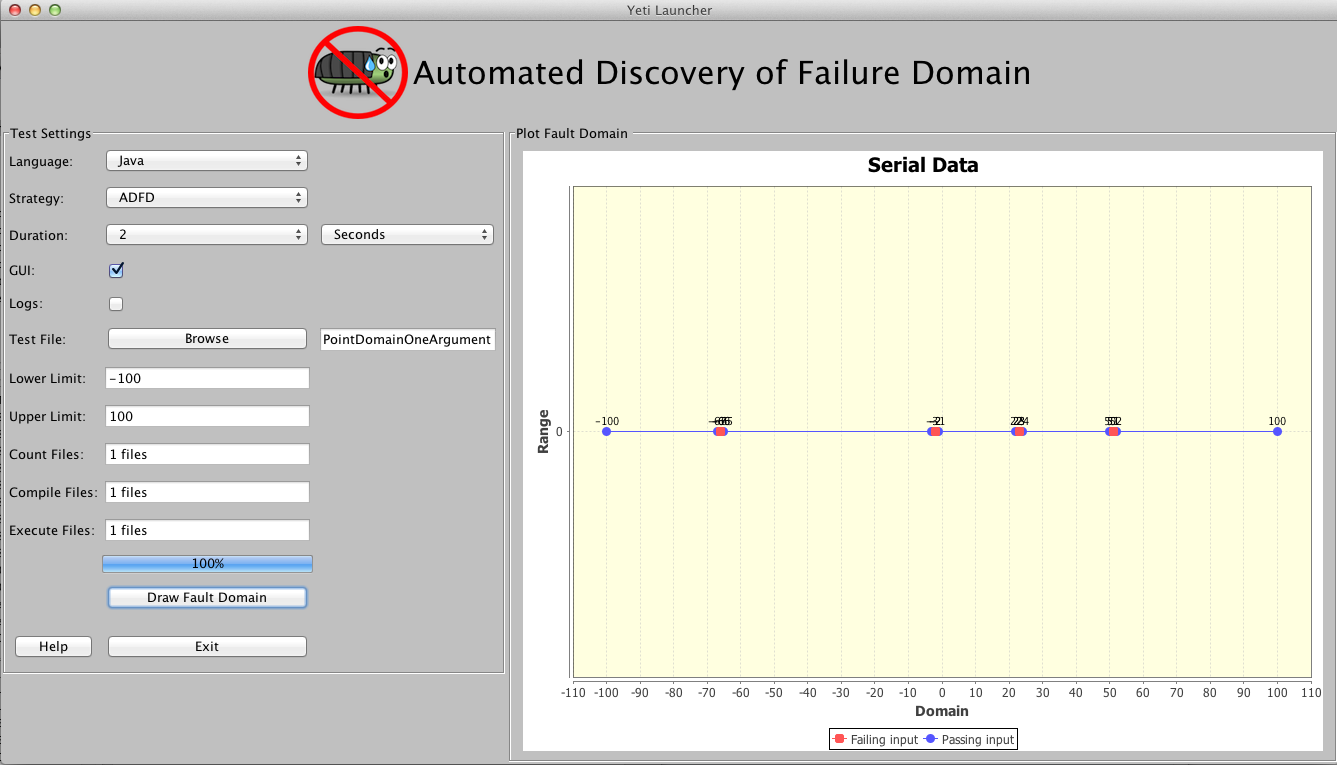
\includegraphics[width=12cm,height=6.6cm]{ADFD/ADFD-front-end.png}
\caption{Front-end of ADFD strategy}
\label{fig:ADFD}
\end{center}
\end{figure}

\noindent \textbf{GUI front-end for providing input:}\\*
\indent ADFD strategy is provided with an easy to use GUI front-end to get input from the user. It takes YETI specific input including language of the program, strategy, duration, enable or disable YETI GUI, logs and a program to test in the form of java byte code. In addition it also takes minimum and maximum values to search for fault domain in the specified range. Default range for minimum and maximum is Integer.MIN\_INT and Integer.MAX\_INT respectively.\\

\noindent \textbf{Automated finding of fault:}\\*
\indent To find the failure domain for a specific fault, the first requirement is to identify that fault in the system. ADFD strategy extends R+ strategy and rely on R+ strategy to find the first fault. Random+ (R+) is an improvement over random strategy with preference to the boundary values to provide better fault finding ability. ADFD strategy is implemented in YETI tool which is famous for its simplicity, high speed and proven ability of finding potentially hazardous faults in many systems \cite{Oriol2011},  \cite{Oriol2012}. YETI is quick and can call up to one million instructions in one second on Java code. It is also capable of testing VB.Net, C, JML and CoFoJa beside Java. \\

\noindent \textbf{Automated generation of modules:}\\*
\indent  After a fault is found in the SUT, ADFD strategy generate complete new Java program to search for fault domains in the given SUT.  These programs with ``.java" extensions are generated through dynamic compiler API included in Java 6 under javax.tools package. The number of programs generated can be one or more, depending on the number of arguments in the test module i.e. for module with one argument one program is generated, for two argument two programs and so on. To track fault domain the program keeps one or more than one argument constant and only one argument variable in the generated program.\\

\noindent \textbf{Automated compilation and execution of modules to discover domains:}\\*
\indent  The java modules generated in previous step are compiled using ``javac *" command to get their binary ``.class" files. The ``java *" command is applied to execute the compiled programs. During execution the constant arguments of the module remain the same but the variable argument receive all the values in range, from minimum to maximum, specified in the beginning of the test. After execution is completed we get two text files of ``Pass.txt" and ``Fail.txt". Pass file contains all the values for which the modules behave correctly while fail file contains all the values for which the modules fail.\\

\noindent \textbf{Automated generation of graph showing domains:}\\*
\indent The values from the pass and fail files are used to plot (x, y) chart using JFreeChart. JFreeChart is a free open-source java library that helps developers to display complex charts and graphs in their applications \cite{Gilbert2008}. Green colour lines with circle represents pass values while red colour line with squares represents the fail values. Resultant graph clearly depicts both the pass and fail domain across the specified input domain. The graph shows red points in case the program fails for only one value, blocks when the program fails for multiple values and strips when a program fails for a long range of values.%\subsection{Flow Chart of the process}

%The following flow chart clearly identify the workflow of the whole process and the various steps involved in the process.

%\begin{figure}[p]
%\centering
%\includegraphics[width=8cm,height=12cm]{automatedFail.png}
%\caption{Automated discovery of Failure Domain}
%\label{fig:autofail}
%\end{figure}




%We found that it is better for the developer to see the range because the fault can be found once but it can generate errors at multiple locations.like point pattern in the first graph only generate fault at location 0 but if the same zero is assigned to second argument then the whole domain values can fail.\\


%\begin{figure}[htp]
%\centering
%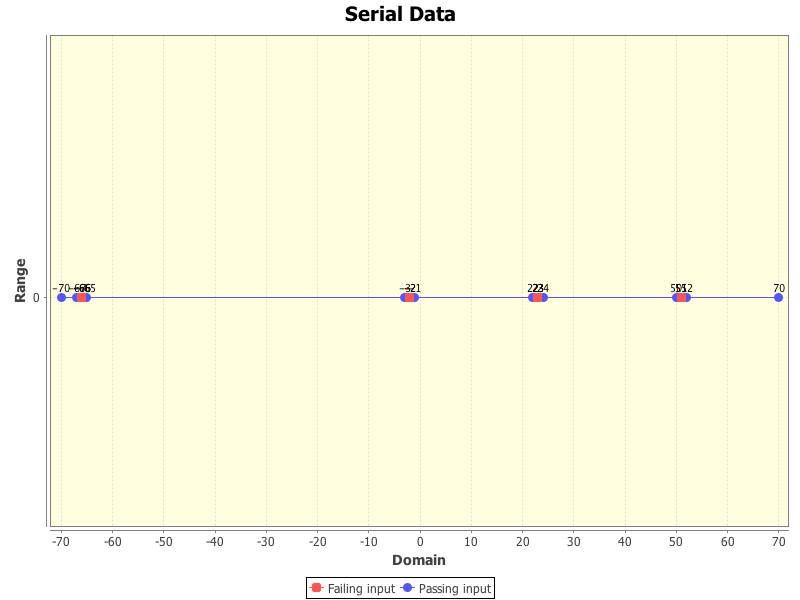
\includegraphics[width=8.5cm,height=6cm]{oneArgumentPointDomain.png}
%\caption{Point pattern failure domain}
%\label{fig:patterns}
%\end{figure}


%Figure \ref{fig:point} shows the example of point pattern. In sub figure \ref{fig1:a} test only fails for 0 out of the whole integer range where as in sub figure \ref{fig1:b} all test fails when static variable is assigned with 0 value.


%\begin{figure}[htp]
%\centering
%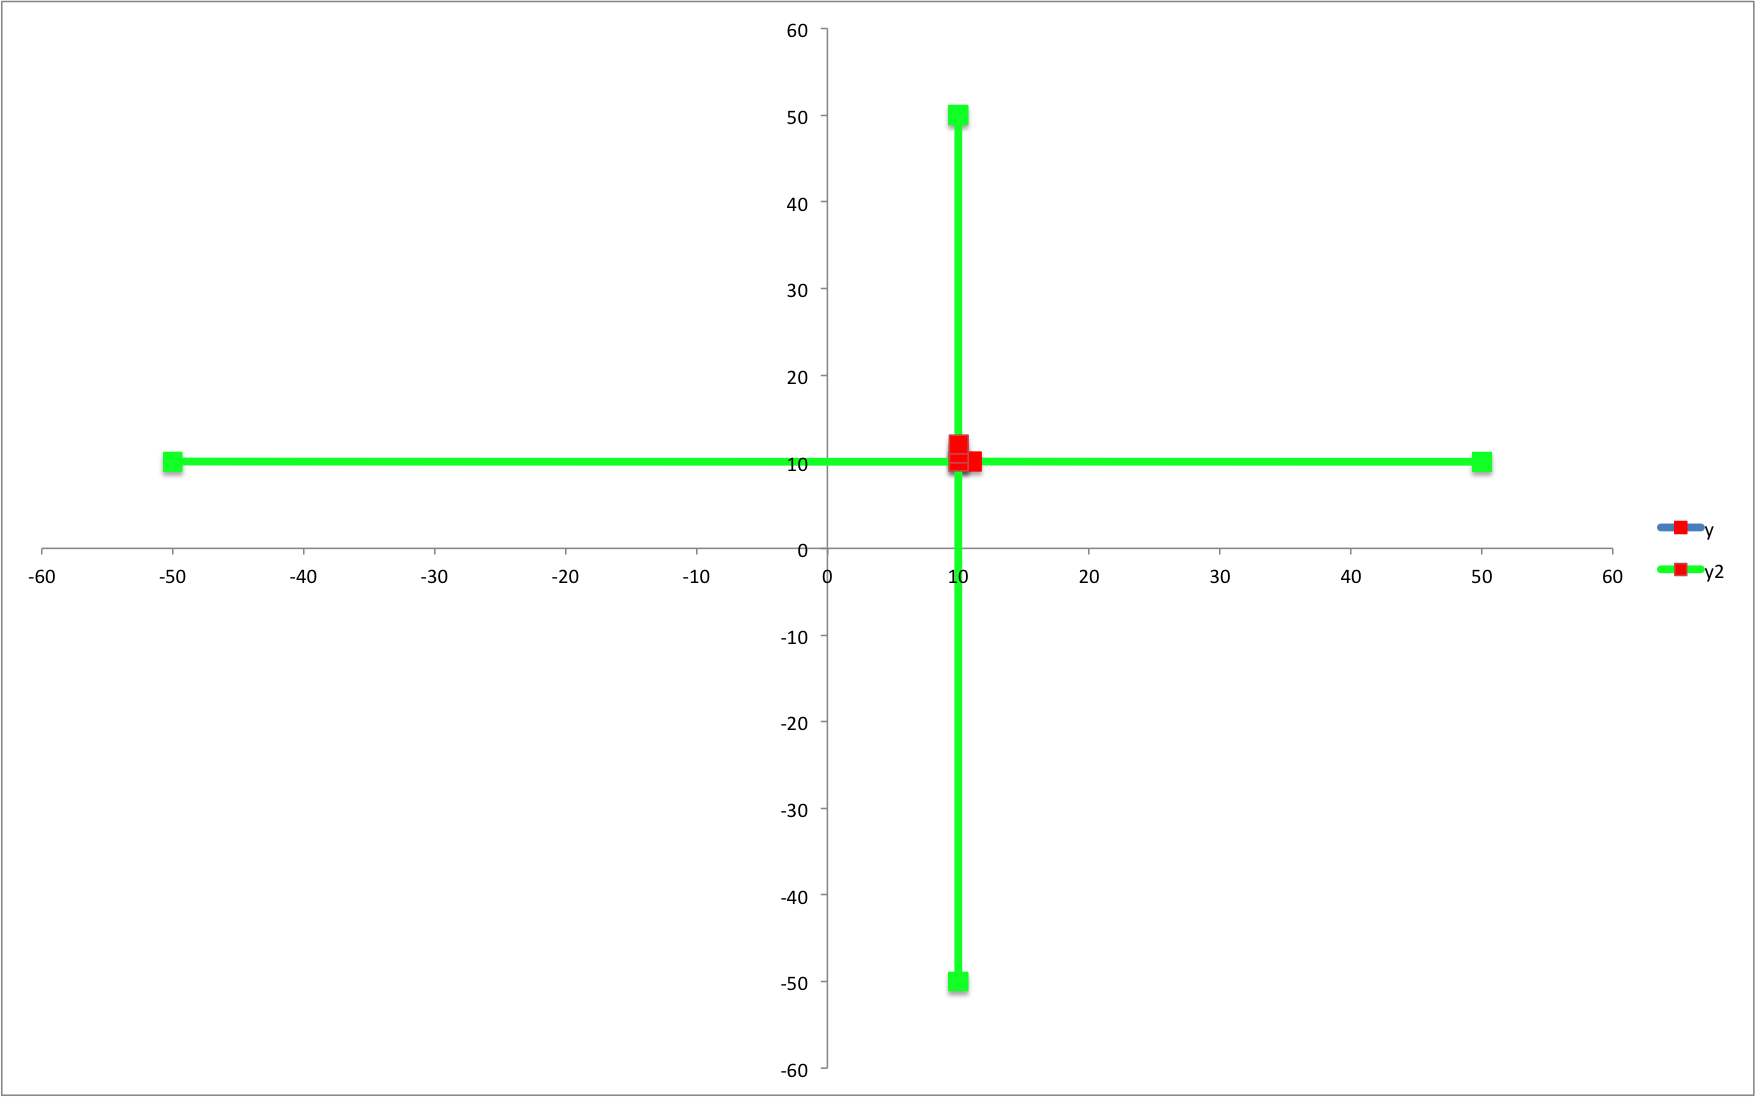
\includegraphics[width=4cm,height=4cm]{block_pattern.png}
%\caption{Block pattern failure domain}
%\label{fig:patterns}
%\end{figure}


%Figure \ref{fig:block} shows the example of block pattern. Both sub figure \ref{fig1:a} and \ref{fig1:b} shows the block pattern of failure. The failure values are given in table \ref{tb:failtable}.

%\begin{figure}[htp]
%\centering
%\begin{center}
%  % Maximum length
 %\subfloat[Test 1 A]{\label{fig1:a}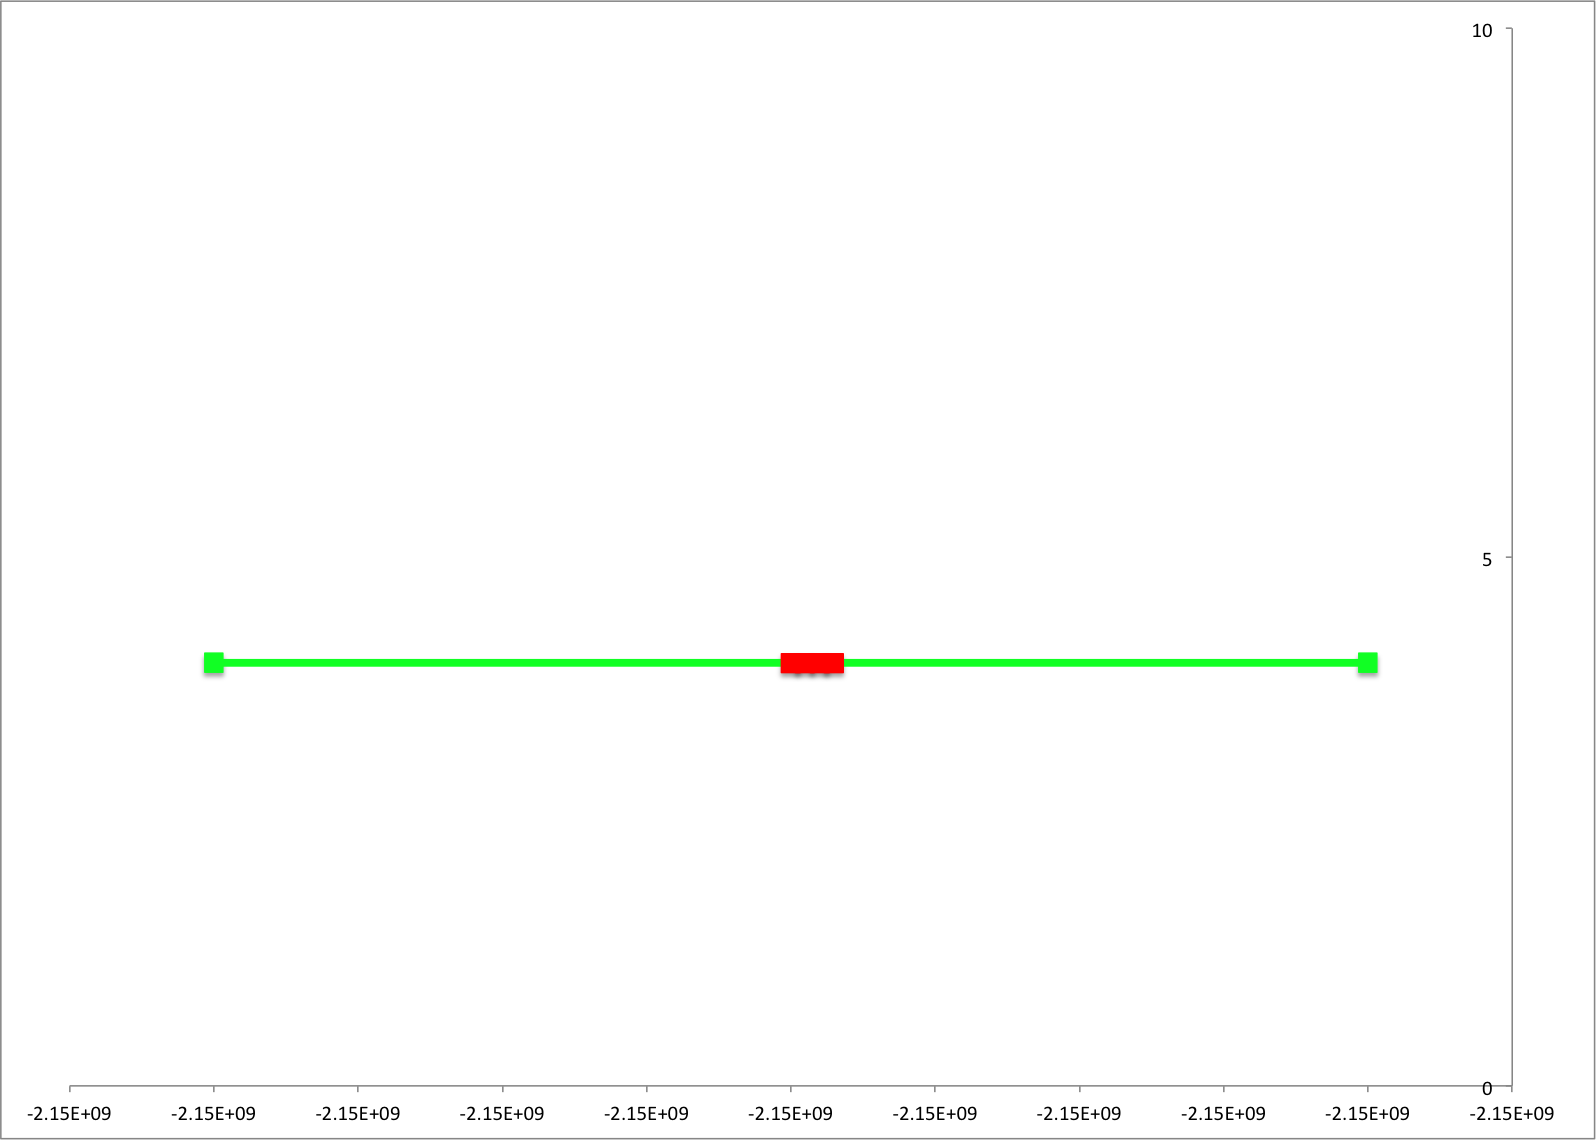
\includegraphics[width=0.49\linewidth]{excel_png/strip_pattern_B.png}}\hfill
 %\subfloat[Test 1 B]{\label{fig1:b}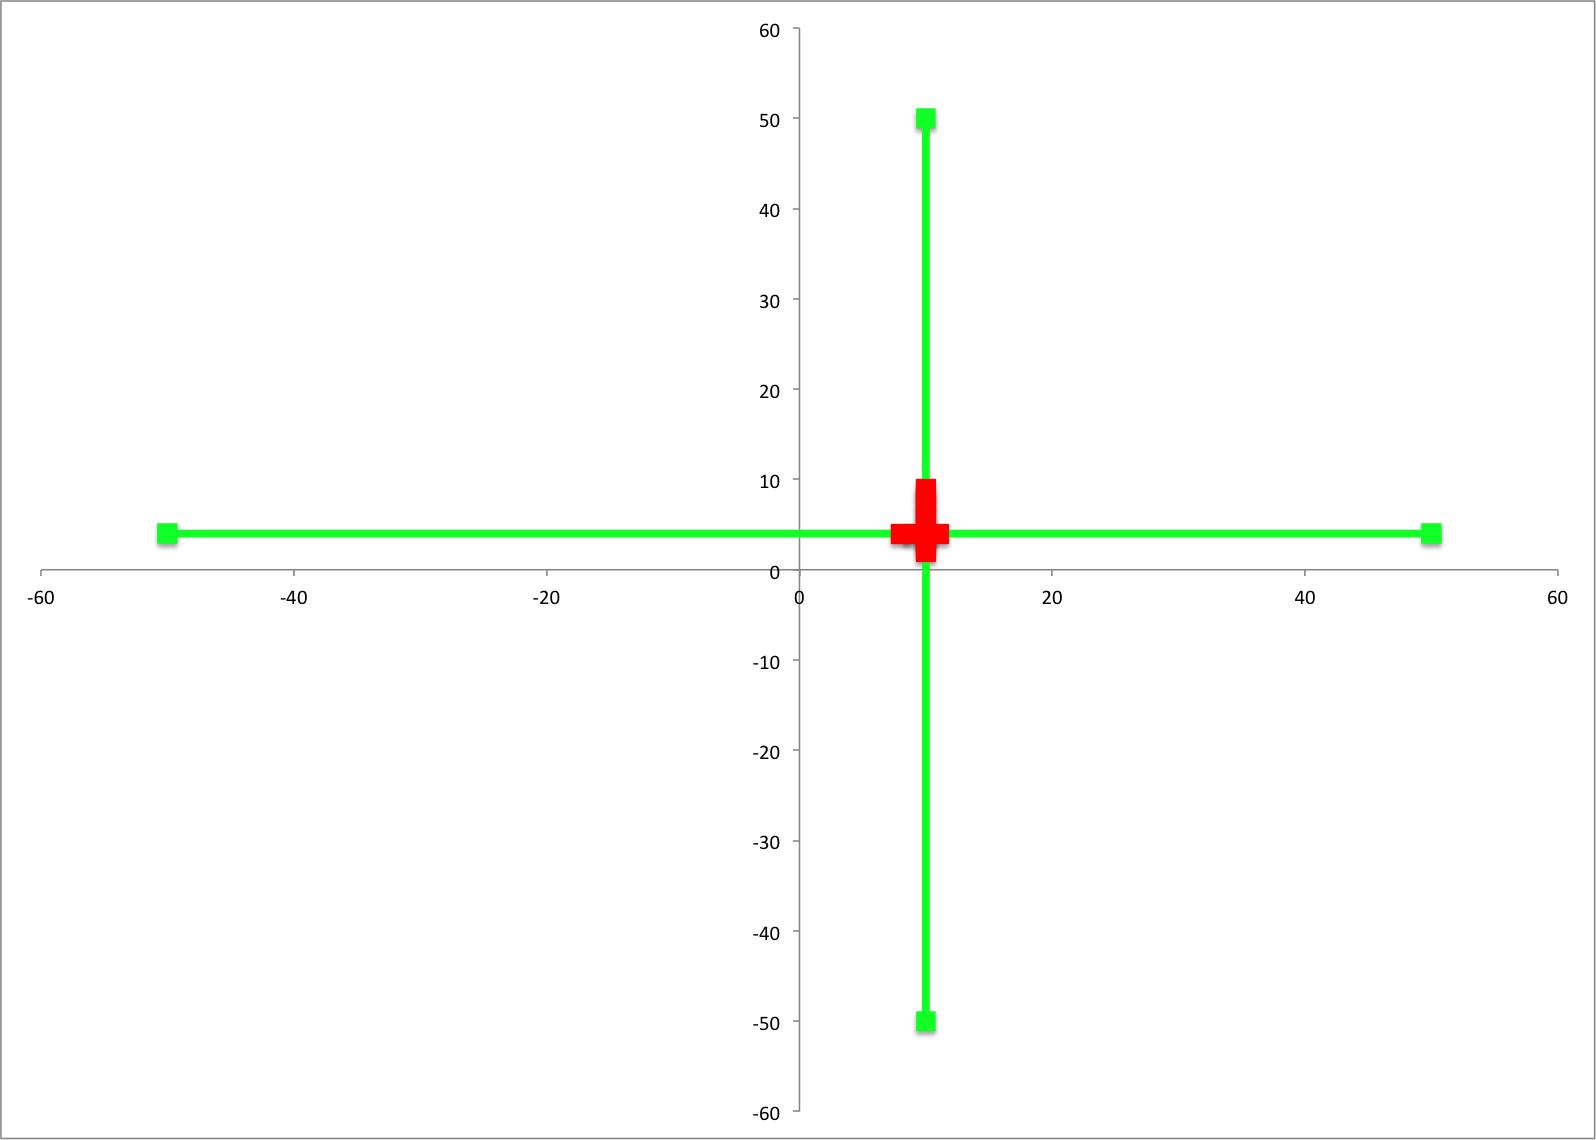
\includegraphics[width=0.49\linewidth]{excel_png/strip_pattern_A.png}}
%  end{center}
%\caption{Strip pattern failure domain}
%%  \label{fig:strip}
%\end{figure}

%Figure shows the example of strip pattern. Here we have two strip failure pattern for test 1 shown in \ref{fig1:a} and \ref{fig1:b} while 1 other for test 2 given in . The failure values are given in table .\\

\section{Implementation}\label{sec:implementation}
The ADFD strategy is implemented in a tool called York Extensible Testing Infrastructure (YETI). YETI is available in open-source at \url{http://code.google.com/p/yeti-test/}. In this section a brief overview of YETI is given with the focus on the parts relevant to the implementation of ADFD strategy. For integration of ADFD strategy in YETI, a program is used as an example to illustrate the working of ADFD strategy. Please refer to  \cite{Oriol2011},  \cite{Oriol2012}, \cite{Oriol2010},  \cite{Oriol2010a},  \cite{Oriol2010b} for more details on YETI tool.

 \subsection{York Extensible Testing Infrastructure}
YETI is a testing tool developed in Java that test programs using random strategies in an automated fashion. YETI meta-model is language-agnostic which enables it to test programs written in functional, procedural and object-oriented languages.

YETI consists of three main parts including core infrastructure for extendibility through specialisation, strategies section for adjustment of multiple strategies and languages section for supporting multiple languages. Both the languages and strategies sections have a pluggable architecture to easily incorporate new strategies and languages making YETI a favourable choice to implement ADFD strategy. YETI is also capable of generating test cases to reproduce the faults found during the test session.
 
 \subsection{ADFD strategy in YETI}
The strategies section in YETI contains all the strategies including random, random+ and DSSR to be selected for testing according to the specific needs. The default test strategy for testing is random. On top of the hierarchy in strategies, is an abstract class YetiStrategy, which is extended by YetiRandomPlusStrategy and it is further extended to get ADFD strategy.
% as shown in figure \ref{fig:hierarchy}. 
 
%\begin{figure}[h]
%\centering
%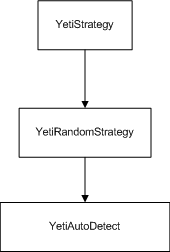
\includegraphics[width=3cm,height=3.5cm]{Hierarchy1.png}
%\caption{Class Hierarchy of automated discovery of failure domains in YETI}
%\label{fig:hierarchy}
%\end{figure}

\subsection{Example}\label{sec:example}
For a concrete example to show how ADFD strategy in YETI proceeds, we suppose YETI tests the following class with ADFD strategy selected for testing. Note that for more clear visibility of the output graph generated by ADFD strategy at the end of test session, we fix the values of lower and upper range by 70 from Integer.MIN\_INT and Integer.MAX\_INT. 

\begin{lstlisting}
/**
 * Point Fault Domain example for one argument
 * @author (Mian and Manuel)
 */
public class PointDomainOneArgument{
	public static void pointErrors (int x){
     		if (x == -66)
       			abort();
     
     		if (x == -2)
     			abort();
      				
     		if (x == 51)
     			abort();
     
     		if (x == 23)
     			abort();
	}
}
\end{lstlisting}

%Published programs from literature \cite{Chen2003}\cite{Chan1996}\cite{Chen2004} of point, block and strip failure patterns are tested to explain the working of ADFD . These programs were translated in to java language for this experiment (See appendix 1 for more details). 

\begin{figure}[H]
\centering
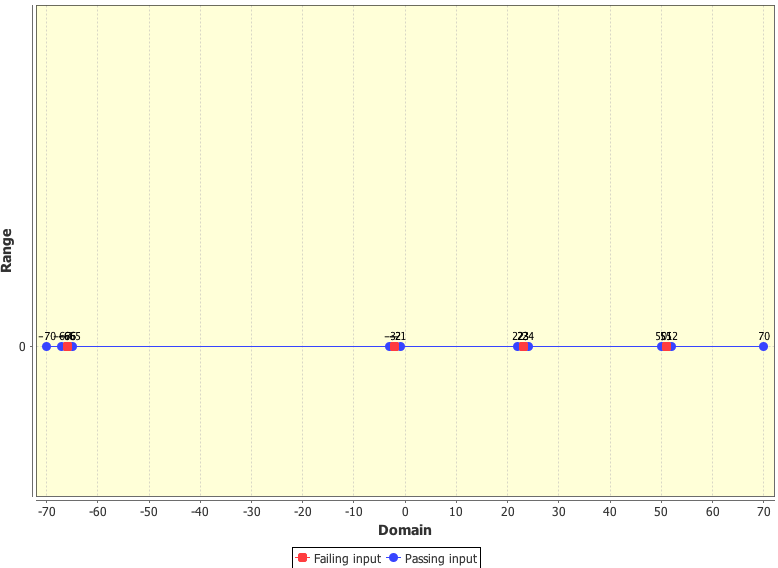
\includegraphics[width=8.2cm,height=3.5cm]{ADFD/pointDomainOneArgument.png}
\caption{ADFD strategy plotting pass and fault domain of the given class}
\label{fig:ADFD-example}
\end{figure}

As soon as any one of the above four faults are discovered the ADFD strategy generate a dynamic program given in Appendix \ref{sec:appendix1} (1). This program is automatically compiled to get binary file and then executed to find the pass and fail domains inside the specified range. The identified domains are plotted on two-dimensional graph. It is evident from the output presented in Figure \ref{fig:ADFD-example} that ADFD strategy not only finds all the faults but also the pass and fail domains.


\begin{comment}
%%%%%% They are commented in this format to decrease the text, for two column format uncomment them.

ADFD can be activated by typing the command java -jar ADFD.jar. After the GUI of ADFD is launched we need to specify yeti specific values that include language of the program under test, strategy for the current test session, duration of test session (minutes or milli-second), display YETI GUI or not and display real time logs or not. Next we browse to select the file for testing and the run button starts testing the file with YETI tool. 

\begin{figure}[ht]
\centering
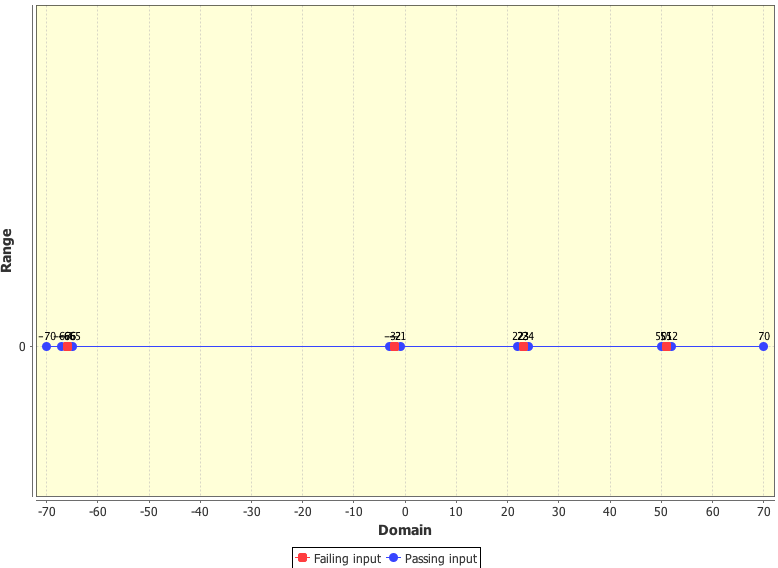
\includegraphics[width=8.2cm,height=5cm]{ADFD/pointDomainOneArgument.png}
\caption{ADFD strategy plotting pass and fault domain of the given class}
\label{fig:ADFD-example}
\end{figure}

In 5 second YETI found one fault out of the above 4 faults. The ADFD strategy in YETI generate a source file (C*.java) at the end of the test session. This file contain the code that searches for fault domains. The count button count the number of files. ADFD create the number of files on the basis of the number of arguments in the method under test. For one argument one method is created and for two argument two methods are created. 

The next button is compile which compile the generated files and generate the byte code (.class files). The execute button execute the byte code and test the method under test for all the values between upper and lower bound. At the end of execution it generates two files (pass.txt and fail.txt). Pass file contain all the values for which the method performed correctly while fail file contain all the values for which the method under test fail.

The draw fault domain button reads the pass and fail files and plot them on the x, y graph where red line with squares show the failing values while the blue line with square shapes show the passing values.
\end{comment}

%%%%%%%%%%%%%%%%%%%%%%%%%%%%%%%%%%%%%%%%%%%%%%%%%%%%%%%%

\section{Experimental Results} \label{sec:experimentalResults}
This section includes the experimental setup and results obtained after using ADFD strategy. Six numerical programs of one and two-dimension were selected. These programs were error-seeded in such a way to get all the three forms of fault domains including point, block and strip fault domains. Each selected program contained various combinations of one or more fault domains. 

All experiments were performed on a 64-bit Mac OS X Lion Version 10.7.5 running on 2 x 2.66 GHz 6-Core Intel Xeon with 6.00 GB (1333 MHz DDR3) of RAM. YETI runs on top of the Java\texttrademark  SE Runtime Environment [version 1.6.0\_35]. 

To elucidate the results, six programs were developed so as to have separate program for one and two-dimension point, block and strip fault domains. The code of selected programs is given in Appendix \ref{sec:appendix1} (2-7). The experimental results are presented in table \ref{sec:fail table} and described under the following three headings.
%\begin{center}

%\end{center}

\begin{table}[h]
%\renewcommand{\arraystretch}{2}
\centering
\scriptsize
%\normalsize

\begin{tabular}{|c|c|c|l|l|l|}

\hline 


\multirow{2}{*}{S. No}	& \multirow{2}{*}{Fault }	 				& \multirow{2}{*}{Module } 		& \multirow{2}{*}{Specific Fault}	 		& \multirow{2}{*}{Pass Domain} 					& \multirow{2}{*}{Fail Domain} 			\\  
					& Domain								&  Dimension					&									&											&								\\ \hline 
\multirow{6}{*}{1} 	&	\multirow{6}{*}{Point}				& 	\multirow{3}{*}{One}			&	\multirow{3}{*}{PFDOneA(i)}	&	-100 to -67, -65 to -3, 		  		& -66, -2, 23, 51			 	\\  
				&									&							&							&	-1 to 50, 2 to 22, 					&							\\  
				&									&							&							&	24 to 50, 52 to 100					&							\\ \cline{3-6}
				&									&	\multirow{3}{*}{Two}			&	\multirow{2}{*}{PFDTwoA(2, i)}	&	(2, 100) to (2, 1),	 				&  (2, 0)						\\  
				&									&							&							&	(2, -1) to (2, -100)					&							\\ \cline{4-6}
				&									& 							&	PFDTwoA(i, 0)				&	Nil								& (-100, 0) to (100, 0)				\\  \hline



\multirow{5}{*}{2} 	&	\multirow{5}{*}{Block}				& 	\multirow{2}{*}{One}			&	\multirow{2}{*}{BFDOneA(i)}	&	-100 to -30, -25 to -2, 					& 	-1 to 1, -29 to -24,		 	\\ 
				&									&							&							&	2 to 50, 55 to 100						&	51 to 54,				\\   \cline{3-6}
				&									&	\multirow{3}{*}{Two}			&	\multirow{2}{*}{BFDTwoA(-2, i)}	&	(-2, 100) to (-2, 20), 					& 	(-2 , 1) to ( -2, 19), 		\\ 
				&									&							&							&      (-2, -1) to (-2, -100)					&	(-2, 0)				\\ \cline{4-6}
				&									& 							&	BFDTwoA(i, 0)				&	Nil								& 	(-100, 0) to (100, 0)		\\  \hline
				
				



\multirow{5}{*}{3} 	&	\multirow{5}{*}{Strip}					& 	\multirow{2}{*}{One}			&	\multirow{2}{*}{SFDOneA(i)}	&	\multirow{2}{*}{-100 to -5, 35 to 100}		& 	\multirow{2}{*}{-4, 34	}\\ 
				&									&							&							&									&				\\  \cline{3-6}
				&									&	\multirow{3}{*}{Two}			&	\multirow{2}{*}{SFDTwoA(-5, i)}	&	(-5, 100) to (-5, 40),					&  (-5, 39) to (-5, 1), 			\\ 
				&									&							&							&	 (-5, 0) to (-5, -100)					&	(-5, 0)				\\ \cline{4-6}
				&									& 							&	SFDTwoA(i, 0)				&	Nil								&  (-100, 0) to (100, 0)			\\  \hline
				
				
\end{tabular}
\bigskip
\caption{Pass and Fail domain with respect to one and two dimensional program}
\label{tab:failtable}
\end{table}




\noindent \textbf{Point Fault Domain:}  Two separate Java programs Pro2 and Pro3 given in Appendix \ref{sec:appendix1} (2, 3) were tested with ADFD strategy in YETI to get the findings for point fault domain in one and two-dimension program. Figure \ref{fig:PFDOne} present range of pass and fail values for point fault domain in one-dimension whereas Figure \ref{fig:PFDTwo} present range of pass and fail values for point fault domain in two-dimension program. The range of pass and fail values for each program in point fault domain are given in (Table \ref{tab:failtable}, Serial No. 1).
%%%%%%%%%%%%%%%%Point Domain%%%%%%%%%%%%%%%%%%%%%%%%%%%%%

\begin{figure} [H]

\subfigure[One dimension module]{
\includegraphics[width=6cm,height=4cm]{ADFD/PFDOne.png}
\label{fig:PFDOne}
}
\subfigure[Two dimension module]{
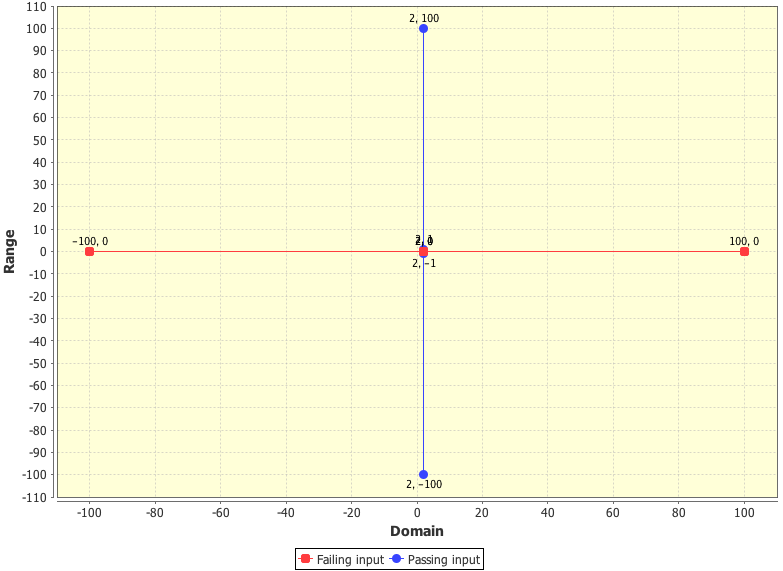
\includegraphics[width=6cm,height=4cm]{ADFD/PFDTwo.png}
\label{fig:PFDTwo}
}


\caption{Chart generated by ADFD strategy presenting point fault domain}
\end{figure}

%\begin{figure}[H]
%\centering
%\includegraphics[width=8.2cm,height=5cm]{PFDOne.png}
%\caption{Chart generated by ADFD strategy presenting point fault domain in one dimension module}
%\label{fig:PFDOne}
%\end{figure}

%\begin{figure}[H]
%\centering
%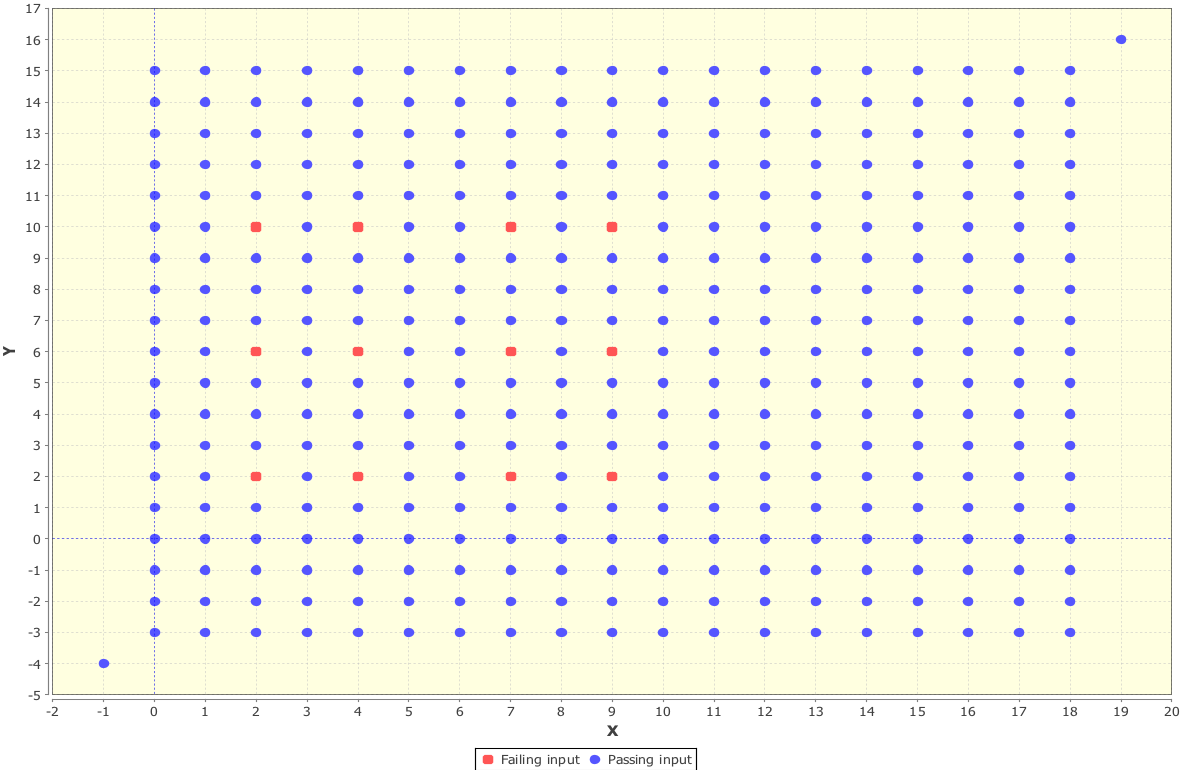
\includegraphics[width=8.2cm,height=5cm]{PFDTwo.png}
%\caption{Chart generated by ADFD strategy presenting point fault domain in two dimension module}
%\label{fig:PFDTwo}
%\end{figure}


\noindent \textbf{Block Fault Domain:}  Two separate Java programs Pro4 and Pro5 given in Appendix \ref{sec:appendix1} (4, 5) were tested with ADFD strategy in YETI to get the findings for block fault domain in one and two-dimension program. Figure \ref{fig:BFDOne} present range of pass and fail values for block fault domain in one-dimension whereas Figure \ref{fig:BFDTwo} present range of pass and fail values for block fault domain in two-dimension program. The range of pass and fail values for each program in block fault domain are given in (Table \ref{tab:failtable}, Serial No. 2).
%%%%%%%%%%%%%%%Block domain %%%%%%%%%%%%%%%%%%%%%%%%%%%%%%
%%%





\begin{figure} [H]

\subfigure[One dimension module]{
\includegraphics[width=6cm,height=4cm]{ADFD/BFDOne.png}
\label{fig:BFDOne}
}
\subfigure[Two dimension module]{
\includegraphics[width=6cm,height=4cm]{ADFD/BFDTwo.png}
\label{fig:BFDTwo}
}


\caption{Chart generated by ADFD strategy presenting block fault domain}
\end{figure}


%\begin{figure}[H]
%\centering
%\includegraphics[width=8.2cm,height=5cm]{BFDOne.png}
%\caption{Chart generated by ADFD strategy presenting block fault domain in one dimension module}
%\label{fig:BFDOne}
%\end{figure}


%\begin{figure}[H]
%\centering
%\includegraphics[width=8.2cm,height=5cm]{BFDTwo.png}
%\caption{Chart generated by ADFD strategy presenting block fault domain in two dimension module}
%\label{fig:BFDTwo}
%\end{figure}



\noindent \textbf{Strip Fault Domain:} Two separate Java programs Pro6 and Pro7 given in Appendix \ref{sec:appendix1} (6, 7) were tested with ADFD strategy in YETI to get the findings for strip fault domain in one and two-dimension program. Figure \ref{fig:SFDOne} present range of pass and fail values for strip fault domain in one-dimension whereas Figure \ref{fig:SFDTwo} present range of pass and fail values for strip fault domain in two-dimension program. The range of pass and fail values for each program in strip fault domain are given in (Table \ref{tab:failtable}, Serial No. 3).


%
%%%%%%%%%%%%%%%%%%%%%%Strip domain %%%%%%%%%%%%%%%%%%%%%%%
\begin{figure} [H]

\subfigure[One dimension module]{
\includegraphics[width=6cm,height=4cm]{ADFD/SFDOne.png}
\label{fig:SFDOne}
}
\subfigure[Two dimension module]{
\includegraphics[width=6cm,height=4cm]{ADFD/SFDTwo.png}
\label{fig:SFDTwo}
}


\caption{Chart generated by ADFD strategy presenting Strip fault domain}
\end{figure}






%\begin{figure}[H]
%\centering
%\includegraphics[width=8.2cm,height=5cm]{SFDOne.png}
%\caption{Chart generated by ADFD strategy presenting strip fault domain in one dimension module}
%\label{fig:SFDOne}
%\end{figure}

%\begin{figure}[H]
%\centering
%\includegraphics[width=8.2cm,height=5cm]{SFDTwo.png}
%\caption{Chart generated by ADFD strategy presenting strip fault domain in two dimension module}
%\label{fig:SFDTwo}
%\end{figure}



\section{Discussion} \label{sec:discussion}

ADFD strategy with a simple graphical user interface is a fully automated process to identify and plot the pass and fault domains on the chart. Since the default settings are all set to optimum the user needs only to specify the module to be tested and click ``Draw fault domain" button to start test execution. All the steps including Identification of fault, generation of dynamic java program to find domain of the identified fault, saving the program to a permanent media, compiling the program to get its binary, execution of binaries to get pass and fail domain and plotting these values on the graph are done completely automated without any human intervention.

In the experiments (section \ref{sec:experimentalResults}), the ADFD strategy effectively identified faults and faults domain in a program. Identification of fault domain is simple for one and two dimension numerical program but the difficulty increases as the program dimension increases beyond two. Similarly no clear boundaries are defined for non-numerical data therefore it is not possible to plot domains for non-numerical data unless some boundary criteria is defined.

ADFD strategy initiate testing with random+ strategy to find the fault and later switch to brute-force strategy to apply all the values between upper and lower bound for finding pass and fault domain. 
It is found that faults at boundary of the input domain can pass unnoticed through ordinary random test strategy but not from ADFD strategy as it scan all the values between lower and upper range.


The overhead in terms of execution time associated with ADFD strategy is dependent mainly on the lower and upper bound. If the lower and upper bound is set to maximum range (i.e. minimum for int is Integer.MIN\_INT and maximum Integer.MAX\_INT) then the test duration is maximum. It is rightly so because for identification of fault domain the program is executed for every input available in the specified range. Similarly increasing the range also shrinks the produced graph making it difficult to identify clearly point, block and strip domain unless they are of considerable size. Beside range factor, test duration is also influenced by the identification of the fault and the complexity of module under test.

ADFD strategy can help the debuggers in two ways. First, it reduces the to and from movement of the project between the testers and debuggers as it identity all the faults in one go. Second, it identifies locations of all fault domains across the input domain in a user-friendly way helping debugger to fix the fault keeping in view its all occurrences.


\section{Threats to Validity} \label{sec:validity}
The major external threat to the use of ADFD strategy on commercial scale is the selection of small set of error-seeded programs of only primitive types such as integer used in the experiments. However, the present study will serve as foundation for future work to expand it to general-purpose real world production application containing scalar and non-scalar data types.

Another issue is the easy plotting of numerical data in the form of distinctive units, because it is difficult to split the composite objects containing many fields into units for plotting. Some work has been done to quantify composite objects into units on the basis of multiple features\cite{Ciupa2006},to facilitate easy plotting. Plotting composite objects is beyond the scope of the present study. However, further studies are required to look in to the matter in depth. 

Another threat to validity includes evaluating program with complex and more than two input arguments. ADFD strategy has so far only considered scalar data of one and two-dimensions. However, plotting domain of programs with complex non-scalar and more than two dimension argument is much more complicated and needs to be taken up in future studies.

Finally, plotting the range of pass or fail values for a large input domain (Integer.MIN\_INT to Integer.MAX\_INT) is difficult to adjust and does not give a clearly understandable view on the chart. Therefore zoom feature is added to the strategy to zoom into the areas of interest on the chart.



\section{Related Works} \label{sec:relatedWork}
Traditional random testing is quick, easy to implement and free from any bias. In spite of these benefits, the lower fault finding ability of traditional random testing is often criticised \cite{Offutt1996}, \cite{Myers2011}. To overcome the performance issues without compromising on its benefits, various researchers have altered its algorithm as explained in section 1. Most of the alterations are based on the existence of faults and fault domains across the input domain \cite{Chan1996}. 

Identification, classification of pass and fail domains and visualisation of domains have not received due attention of the researchers. Podgurski et. al., \cite{Podgurski2003} proposed a semi-automated procedure to classify similar faults and plot them by using a Hierarchical Multi Dimension Scaling (HMDS) algorithm. A tool named Xslice \cite{Agrawal1995} visually differentiates the execution slices of passing and failing part of a test. Another tool called Tarantula uses colour coding to track the statements of a program during and after the execution of the test suite \cite{Jones2002}. A serious limitation of the above mentioned tools is that they are not fully automated and require human interaction during execution. Moreover these tools are based on the already existing test cases where as ADFD strategy generate test cases, discover faults, identify pass and fault domains and visualise them in a fully automated manner. 


\section{Conclusion} \label{sec:conclusion}

Results of the experiments (section 4), based on applying ADFD strategy to error-seeded numerical programs provide, evidence that the strategy is highly effective in identifying the faults and plotting pass and fail domains of a given SUT. It further suggests that the strategy may prove effective for large programs. However, it must be confirmed with programs of more than two-dimension and different non-scalar argument types. ADFD strategy can find boundary faults quickly as against the traditional random testing, which is either, unable or takes comparatively long time to discover the faults.

The use of ADFD strategy is highly effective in testing and debugging. It provides an easy to understand test report visualising pass and fail domains. It reduces the number of switches of SUT between testers and debuggers because all the faults are identified after a single execution. It improves debugging efficiency as the debuggers keep all the instances of a fault under consideration when debugging the fault.

}

\ychapter{Directed Random Plus Strategy}{Directed Random Plus Strategy\label{CHAP:DRPS}}{\input{DirectedRandomPlusStrategy}}

%% The chapter on the use of knowledge-based admissible models in PAC-MDP learning
%\ychapter{Evaluation on Artificial Corpus}{Evaluation on Artificial
%Corpus\label{CHAP:PACMDPADMISSMODELS}}{\input{PACMDP_Admissible_Models}}

%% The chapter on the Analysis of Eligibility Traces
%\ychapter{Analysis of Exploration with Eligibility Traces}{Analysis of Exploration with Eligibility Traces\label{CHAP:ELTRACES}}{\input{Eligibility_Traces_Analysis}}

%%conclusion
\ychapter{Conclusion}{Conclusion\label{CHAP:CONCLUSION}}{\section{Conclusion}

The main goal of the present study was to develop a new random strategy which could find more faults in lower number of test cases and shorter execution time. The experimental findings revealed that DSSR strategy was up to 30\% more effective in finding faults as compared to random test strategy. The DSSR strategy not only gave more consistent results but it proved more effective in terms of detecting faults as compared to random testing. However in comparison to random plus strategy both perform equally well in 95% of the experiments but in 5% random plus perform better and faster then DSSR strategy which is due to the fact that programs contain errors in the form of point patterns and adding fault neighbouring values only increases processing without improving results. \\

Improvement in performance of DSSR strategy over random strategy was achieved by taking advantage of Random Plus and fault neighbouring values. Random plus incorporated not only border values but it also added values having higher chances of finding faults in the SUT to the list of interesting values.\\

The DSSR strategy is highly effective in case of systems containing block and strip pattern of failure across the input domain.\\

Due to the additional steps of scanning the list of interesting values for better test values and addition of fault finding test value and its neighbour values, the DSSR strategy takes upto 5\% more time to execute equal number of test cases than pure random testing and 3% more than random plus. \\

In the current version of DSSR strategy, it might depend on random or random plus strategy for finding the first fault if the fault test value was not in the list of interesting values. Once the first fault is found only then DSSR strategy could make an impact on the performance of test strategy.\\

The limitation of random plus strategy is that it maintains a static list of interesting values which remains the same for each program under test, and can be effective in many cases but not always. The better approach will be to have a dynamic list of interesting values that is automatically updated for every program which can be achieved by adding the program literals and its surrounding values to the list of interesting values prior to starting every new test session.




}


% %%%%%%%%%%%%%%%%%%%%% APPENDIX ETC %%%%%%%%%%%%%%%%%%%%%%%%%%%%%%%%%%%%

%\begin{appendix}
%\addcontentsline{toc}{chapter}{Appendices}
%--  \input{desertquestionnaire}
%--  \input{restoquestionnaire}
%--  \input{desertgraph}
%\end{appendix}


% (*) Definitions before glossary. Definitions can be easily done with the nomencl package (used in the thesis template from Cambridge).

% (*) Glossary before references.
% %  \input{}
% %   \yorkGlossary  Terms that require explanation
% %                     shall be defined in a glossary, which shall
% %                     include a key to any abbreviations used. For
% %                     an abbreviation not in common use, the term
% %                     shall be given in full at the first instance
% %                     followed by the abbreviation in brackets.
%   \input{Cglossary}

%\backmatter
%bibtex setup and path names

%latex get crazy if we don't disconnect natbib citeindex
\citeindexfalse
\renewcommand{\bibname}{References}
\bibliographystyle{newapa}
%\bibliography{../../mybib}
\bibliography{mybib}

%\yorkBib{}


% index.bat has to be executed to process index files.
\yorkIndex
\yorkCiteIndex
\yorkNomIndex

\begin{figure}[b]
 \begin{center}
 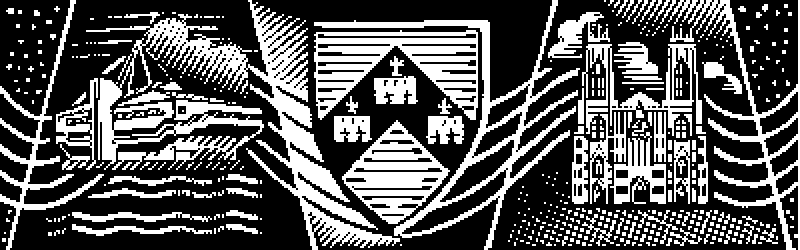
\includegraphics [width=7cm] {Woodcuts/univwoodcut}
\end{center}
\end{figure}

%\ylastpage{
%\begin{picture}(0.0,0.0)
%  \put(80,-550){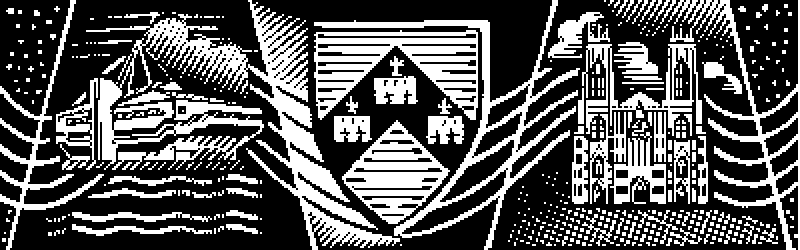
\includegraphics[width=7cm]{Woodcuts/univwoodcut}}
%\end{picture}
%}


%\listoftodos




\end{document}
